\documentclass[11pt,psfig]{article}
\usepackage{epsfig}
\usepackage{times}
\usepackage{amssymb}
\usepackage{float}
\usepackage{listings}
\usepackage{graphicx}
\usepackage{caption}
\usepackage{subcaption}

\newcount\refno\refno=1
\def\ref{\the\refno \global\advance\refno by 1}
\def\ux{\underline{x}}
\def\uw{\underline{w}}
\def\bw{\underline{w}}
\def\ut{\underline{\theta}}
\def\umu{\underline{\mu}} 
\def\bmu{\underline{\mu}} 
\def\be{p_e^*}
\newcount\eqnumber\eqnumber=1
\def\eq{\the \eqnumber \global\advance\eqnumber by 1}
\def\eqs{\eq}
\def\eqn{\eqno(\eq)}

 \pagestyle{empty}
\def\baselinestretch{1.1}
\topmargin1in \headsep0.3in
\topmargin0in \oddsidemargin0in \textwidth6.5in \textheight8.5in
\begin{document}
\setlength{\parskip}{1.2ex plus0.3ex minus 0.3ex}


\thispagestyle{empty} \pagestyle{myheadings} \markright{Crater Lake Reconstruction}

\title{CS 217 Final Project: 3D Reconstruction of Crater Lake}
\author{Zachary DeStefano, 15247592}
\date{Due Date: June 11, 2015}

\maketitle

\vfill\eject

\newpage

\section{Background}

For this project, I attempted a 3D reconstruction of parts of Crater Lake National Park in Oregon.
\begin{figure}[H]
\centering
\includegraphics[width=\columnwidth]{craterLakeWinter.jpg}
\caption{Crater Lake during winter}
\end{figure}
Google Earth offers a 3D view of Crater Lake and my goal was something close to what it showed. There is an island in the middle of the lake called Wizard Island. I decided to focus on that island as well as nearby mountain peaks for my reconstruction. \\
\\
I used pictures taken from different angles in order to do the reconstruction. In order to ensure that I had a wealth of pictures to use, I found high definition video and used a handful of the frames. That way I do not need to worry about using pictures that were taken at different times of the day or year.\\
\\
After looking at multiple high definition videos of Crater Lake, there were two scenes that I decided to attempt to reconstruct. The first one was taken from Merriam Point and it shows Wizard Island as well as nearby peaks. The second one was taken from different points on the surface of the lake and it shows two views of Wizard Island. \\
\\
\newpage

Here are images of Crater Lake via Google Earth

\begin{figure}[H]
\centering
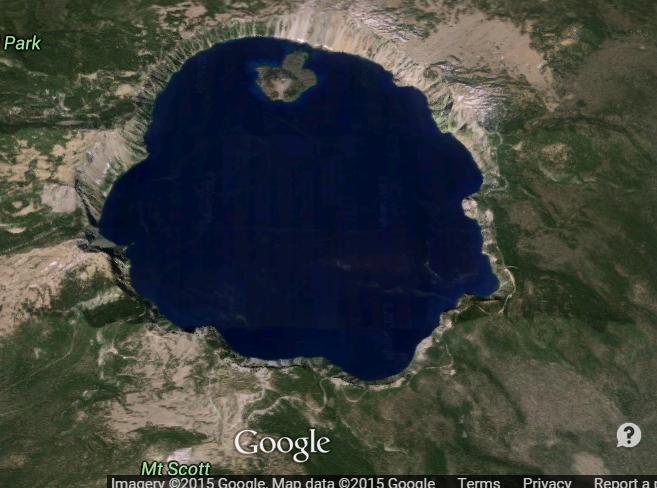
\includegraphics[width=\columnwidth]{googleEarthView1.png}
\caption{Goal Sample: Top View of Crater Lake using Google Earth}
\end{figure}
\begin{figure}[H]
\centering
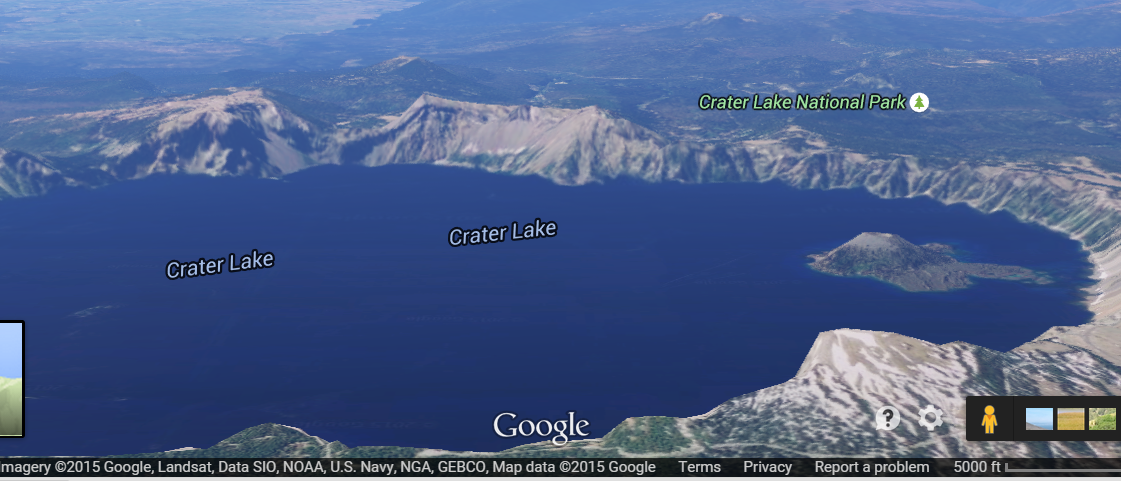
\includegraphics[width=\columnwidth]{googleEarthView2.png}
\caption{Goal Sample: Side View of Crater Lake using Google Earth}
\end{figure}

\newpage

Here are two of the shots from the Merriam Point scene

\begin{figure}[H]
\centering
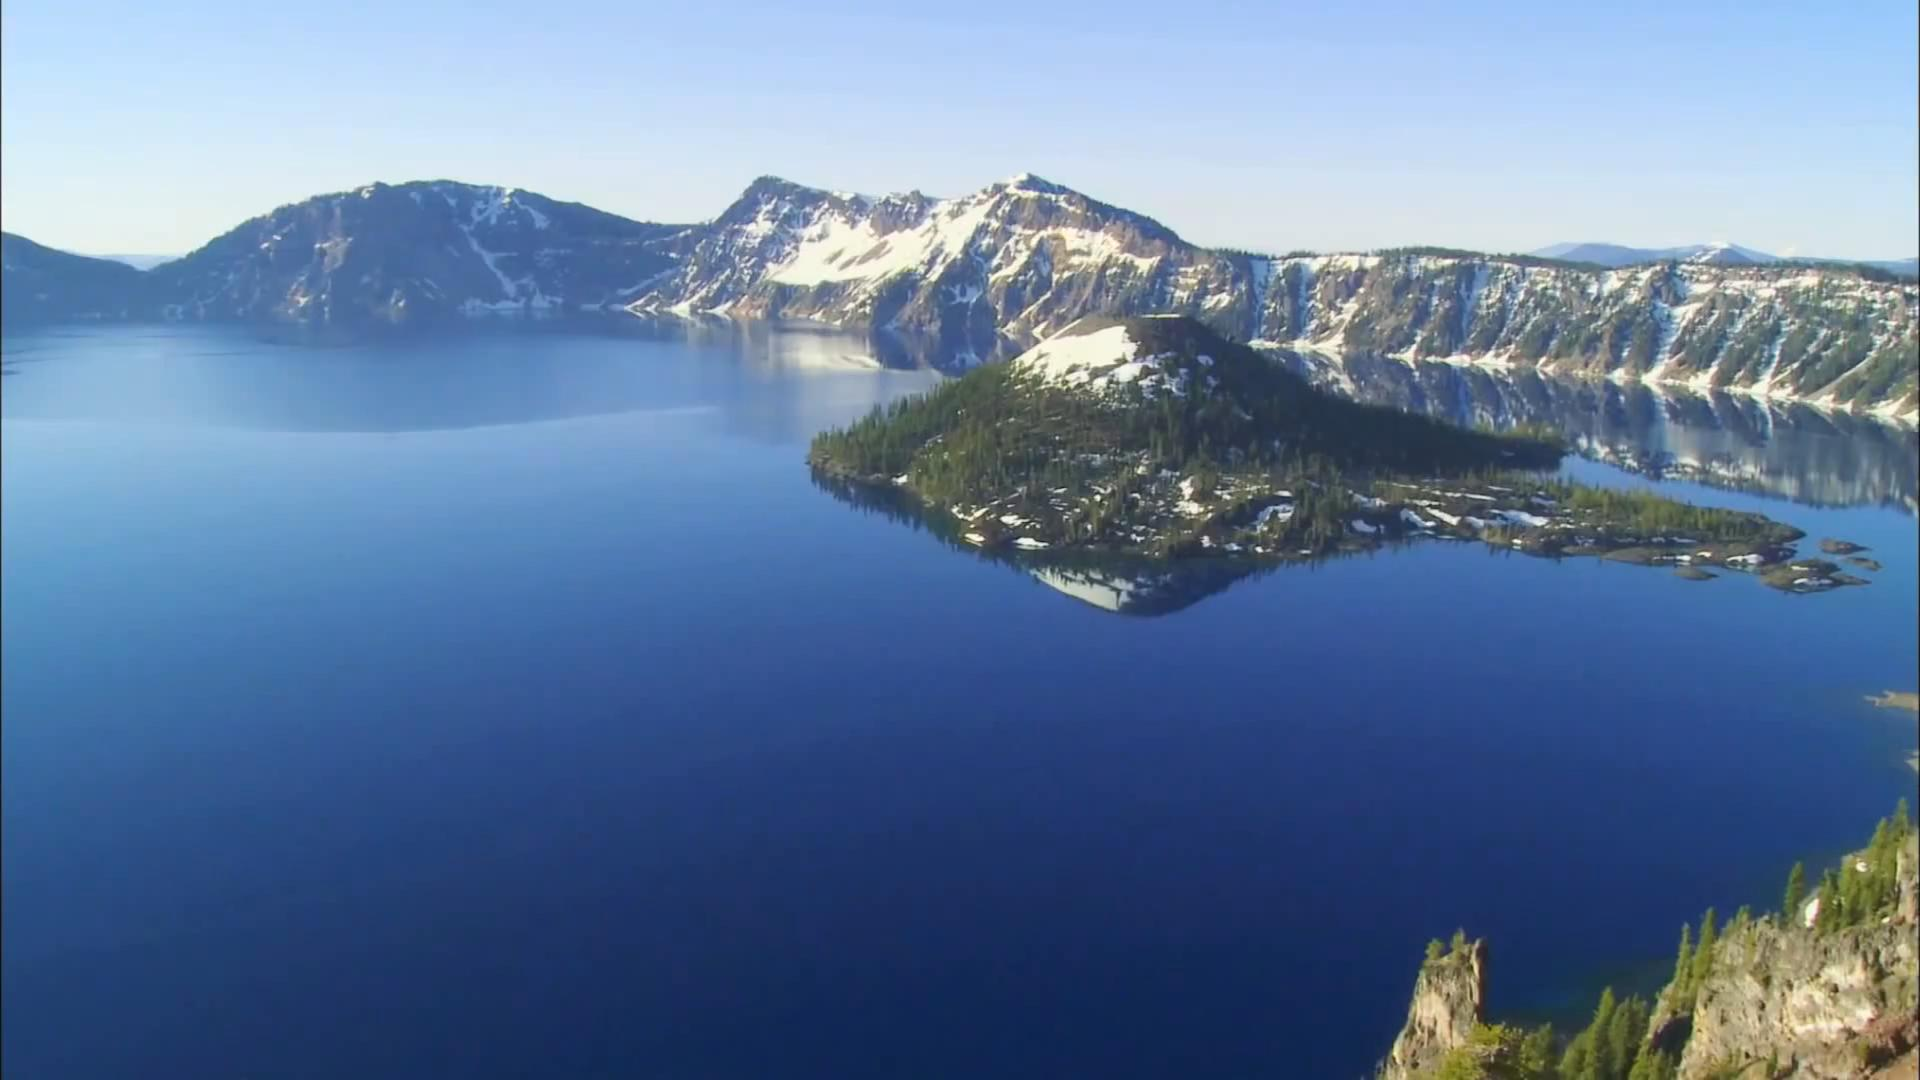
\includegraphics[height=3.5in]{sfmPics1J2/shot4.jpg}
\caption{Merriam Point Scene, Left Camera Shot}
\end{figure}
\begin{figure}[H]
\centering
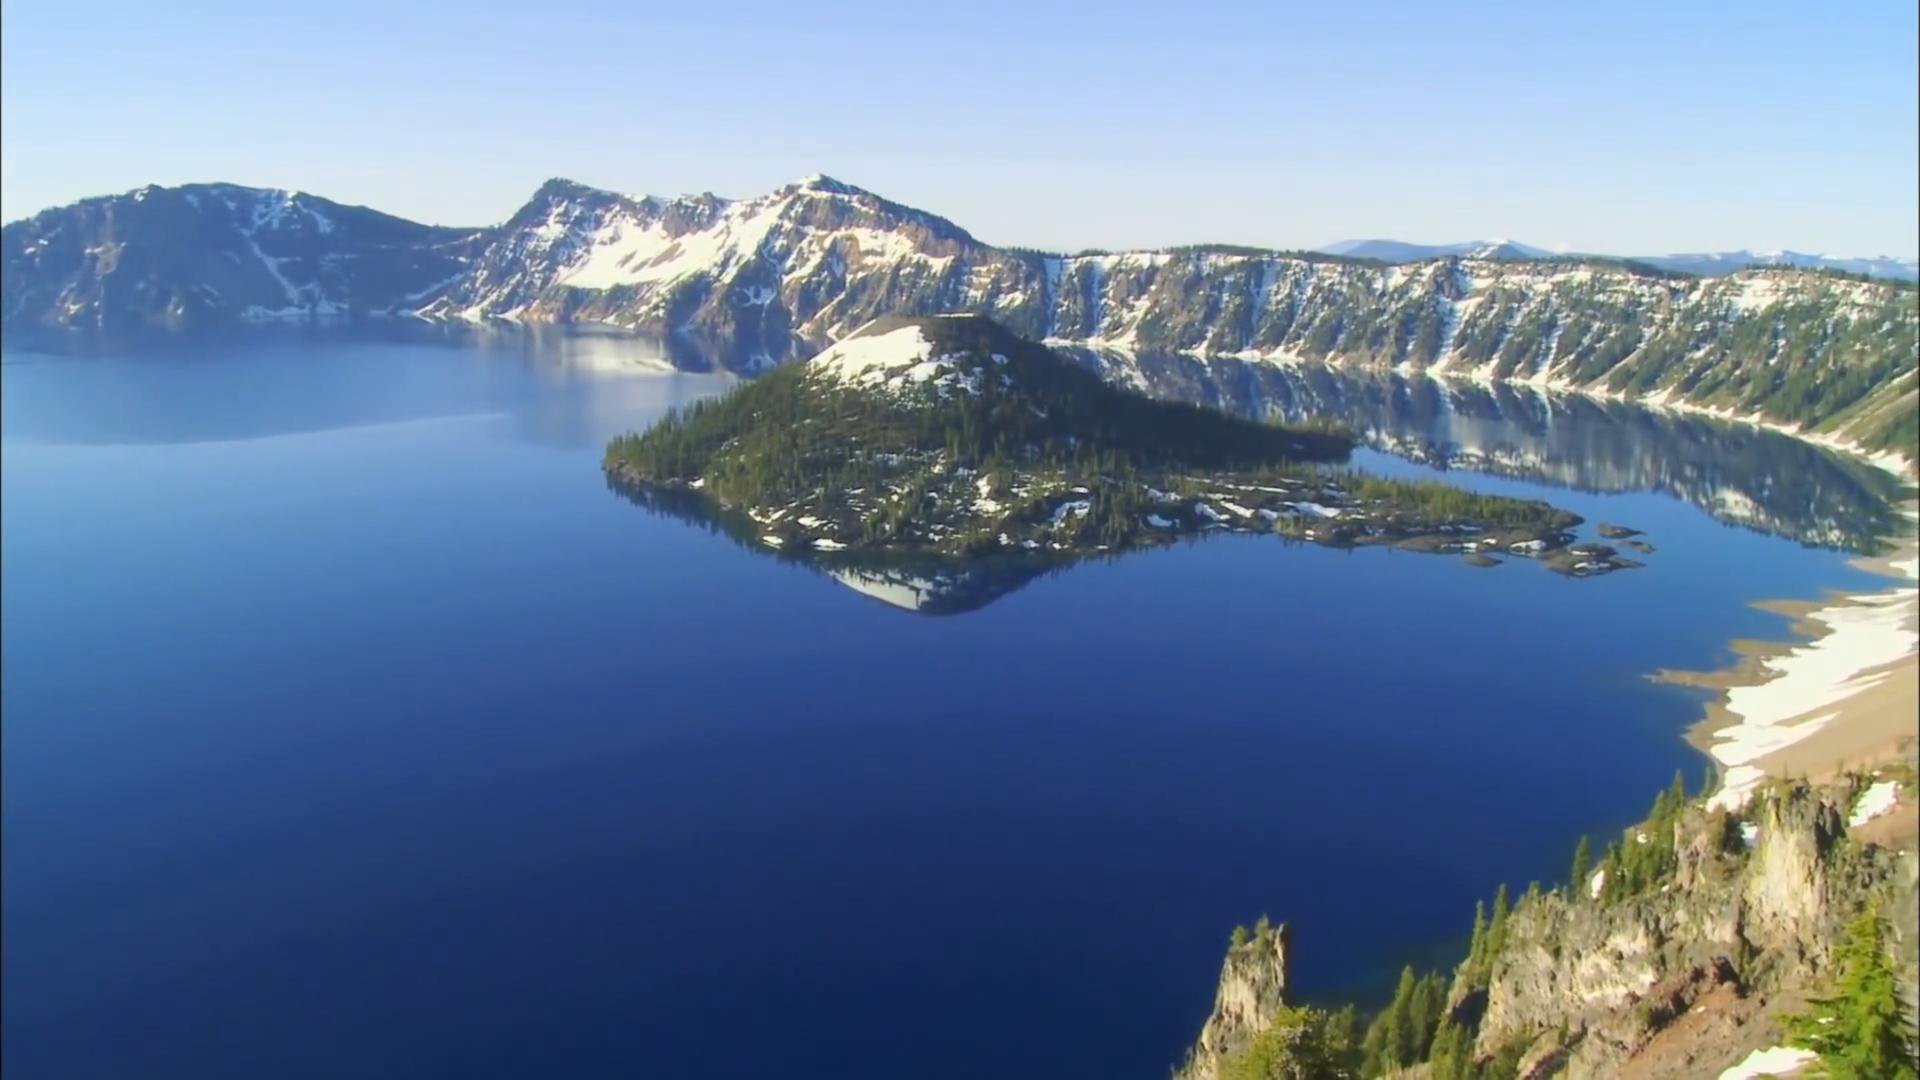
\includegraphics[height=3.5in]{sfmPics1J2/shot26.jpg}
\caption{Merriam Point Scene, Right Camera Shot}
\end{figure}

\newpage

Here are two shots from the other scene showing Wizard Island

\begin{figure}[H]
\centering
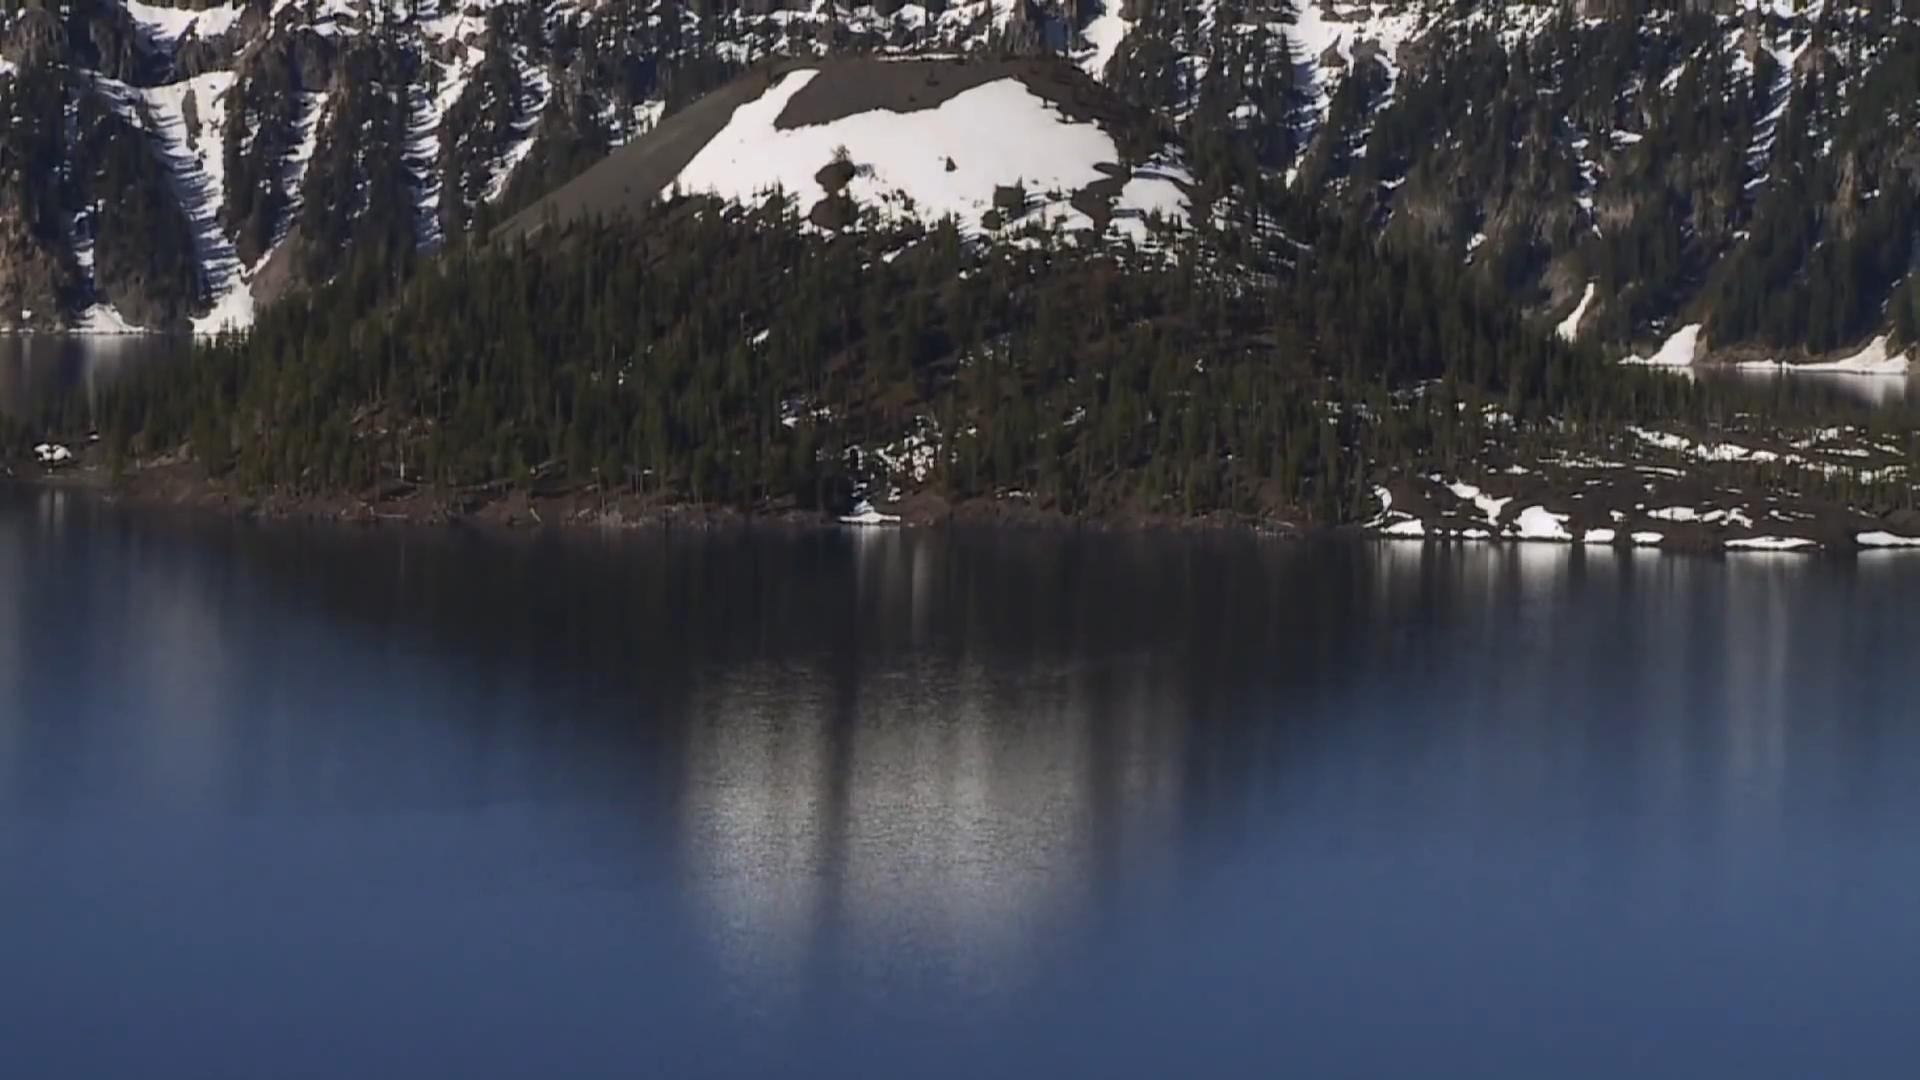
\includegraphics[height=3.5in]{sfmPics3/shot1.jpg}
\caption{Wizard Island Scene, close up shot}
\end{figure}
\begin{figure}[H]
\centering
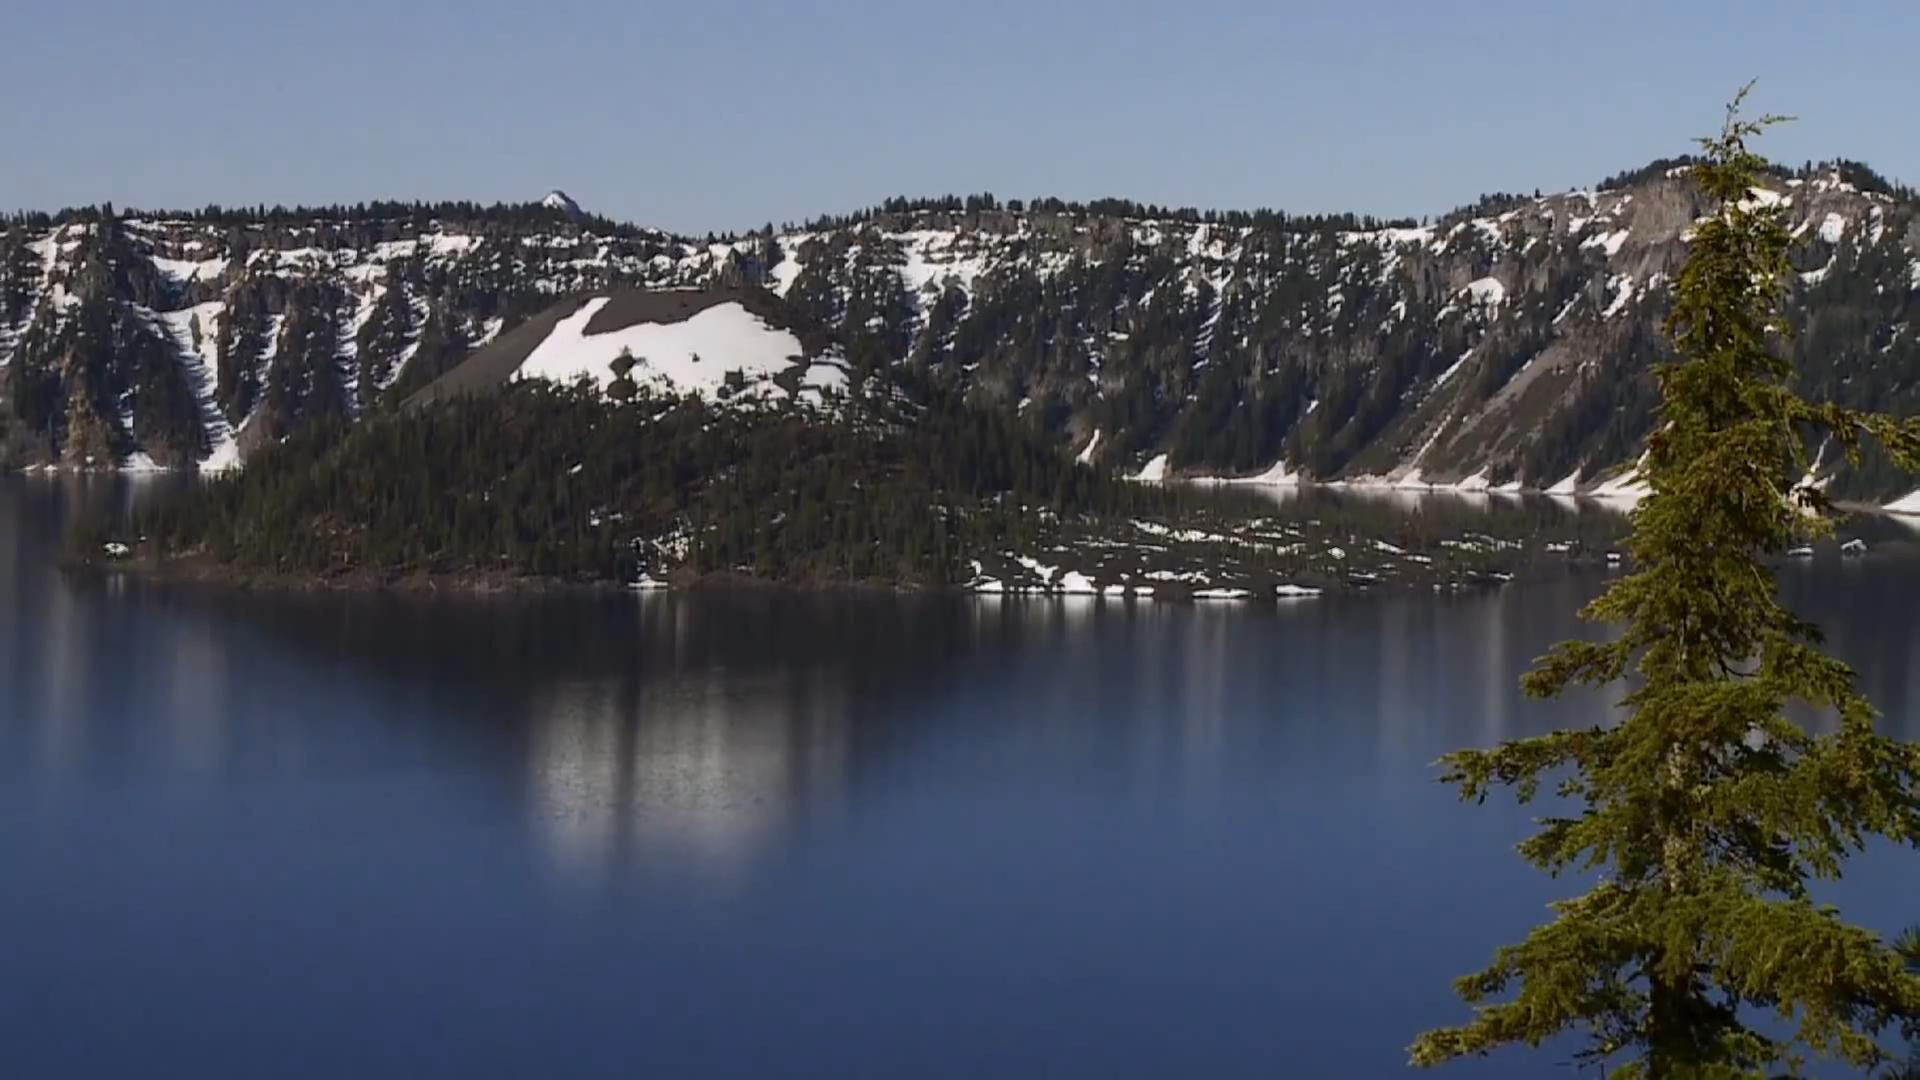
\includegraphics[height=3.5in]{sfmPics3/shot24.jpg}
\caption{Wizard Island Scene, further shot}
\end{figure}

\newpage

\section{Reconstruction of Merriam Point Scene}

To do this reconstruction, I tried Calibration and Triangulation as well as VisualSFM. For calibration, I used a few distinguishable landmarks in the picture. There is existing data already on these landmarks which I used to get the scene 3D points for calibration.  

\subsection{3D Calibration Points}

The points I focused on were various peaks as well as recognizable points on the surface of the lake. These points could easily be spotted in a topographic map. Here is the left camera shot marked with the points used:
\begin{figure}[H]
\centering
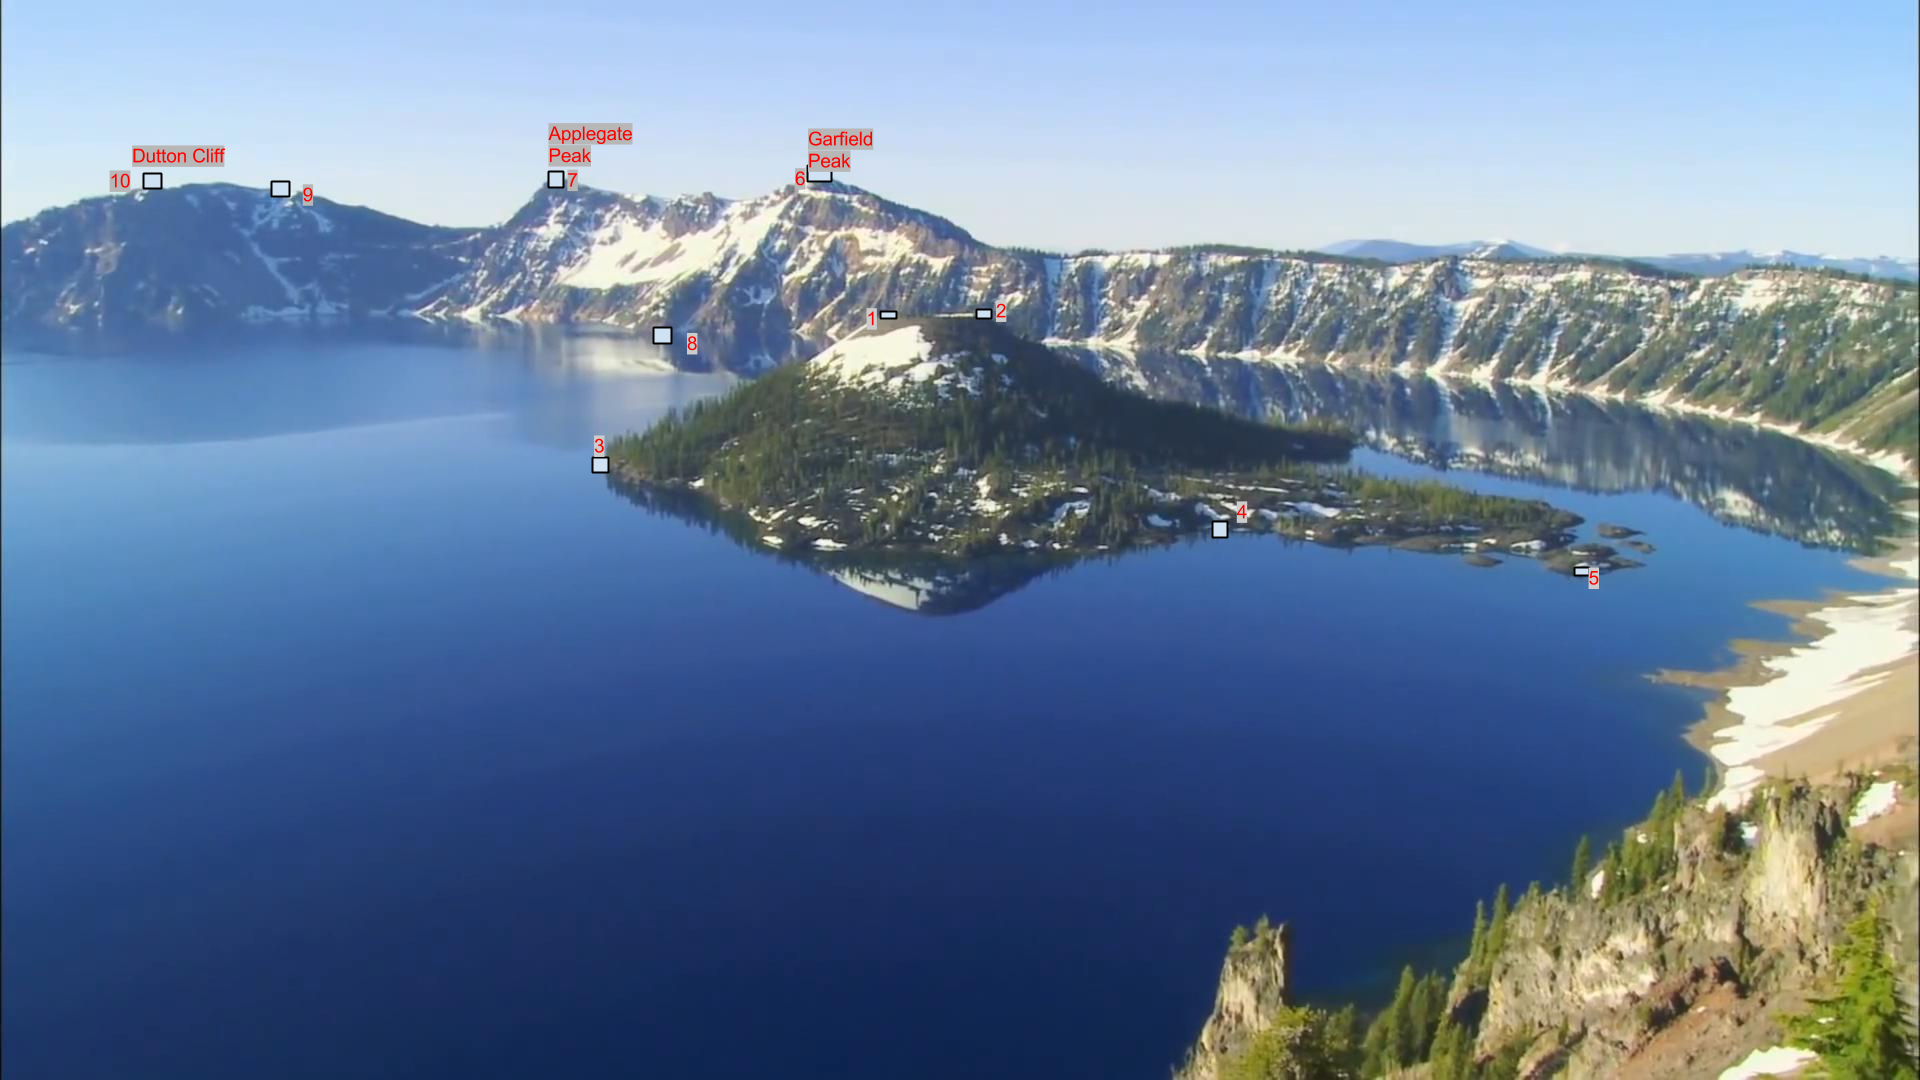
\includegraphics[width=\columnwidth]{sfmResults1/Photo_withPoints.png}
\caption{Left Camera Shot with Calibration Points marked}
\end{figure}

\newpage

Here are the topographic maps for the points shown in the previous picture. 
\begin{figure}[H]
\centering
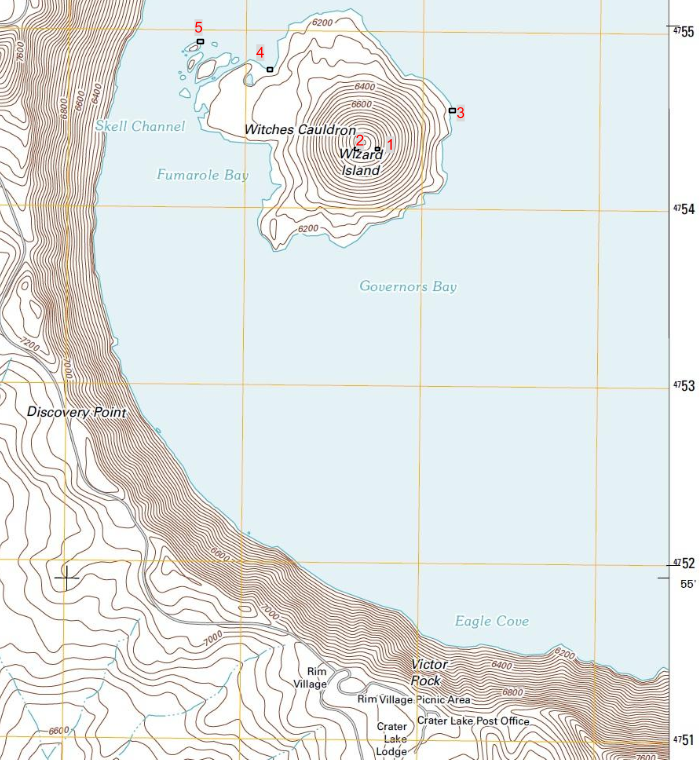
\includegraphics[width=\columnwidth]{sfmResults1/TopMap_withPoints_wizardIsland.png}
\caption{Calibration Points near Wizard Island on Topographic Map}
\end{figure}
\begin{figure}[H]
\centering
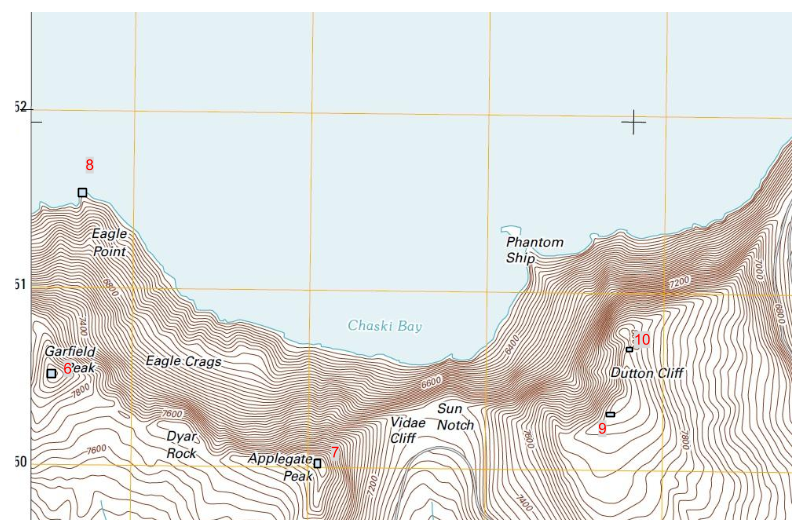
\includegraphics[width=\columnwidth]{sfmResults1/TopMap_withPoints_peaks.png}
\caption{Calibration Points at the peaks on Topographic Map}
\end{figure}

I used the maps to obtain the $x,y$ coordinates for each of my calibration points. I made the origin the point on both maps where the latitude line is labeled 51 and the longitude line is labeled 47. I used the map scale to obtain a conversion from pixels to feet so that my units for the 3D coordinates were in feet.  \\
\\
The z coordinate represented the height in feet. I decided to make the surface of the lake my $z=0$ plane. In order to obtain the z coordinate for my points, I used the following map which showed the exact elevations for each of my points. 
\begin{figure}[H]
\centering
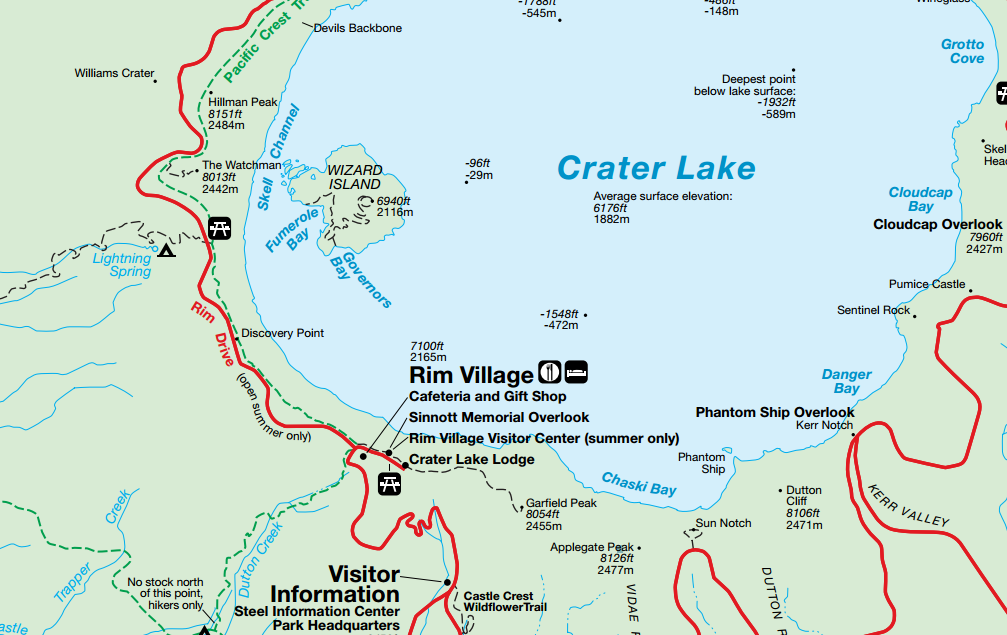
\includegraphics[width=\columnwidth]{sfmResults1/elevationsListed.png}
\caption{Calibration Points with elevations listed}
\end{figure}

\newpage

\subsection{Triangulation using Manually Selected Points}

After calibrating the left and right images, I decided to try triangulating points by manually selecting them in both images and seeing if a good reconstruction could be calculated. I split the points into 3 groups in order to more easily see how good the reconstruction ended up. Here is the left camera shot with the triangulation points. 
\begin{figure}[H]
\centering
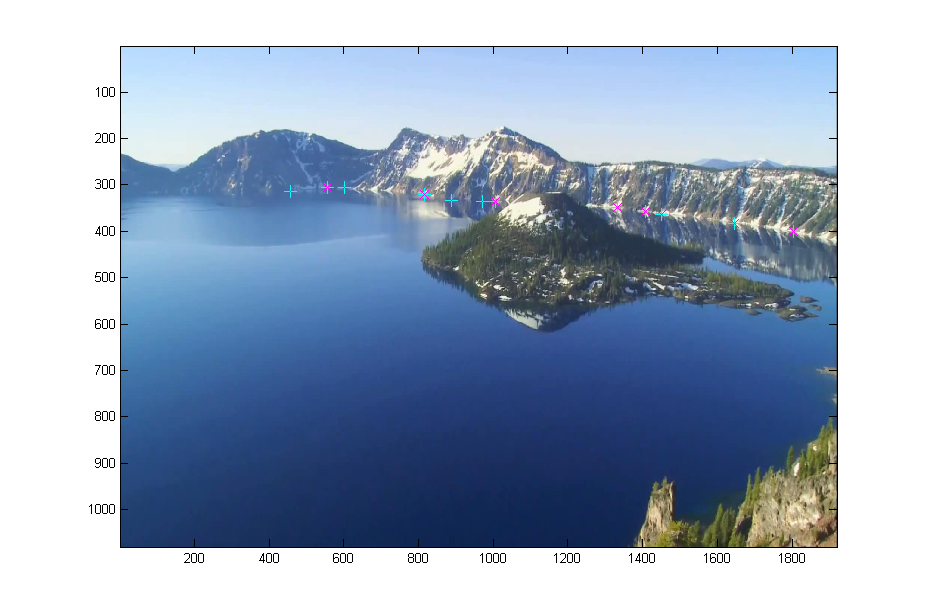
\includegraphics[height=3.5in]{sfmResults1/photoLeft_lakeRidgePoints.png}
\caption{Triangulation Points along the lake}
\end{figure}
\begin{figure}[H]
\centering
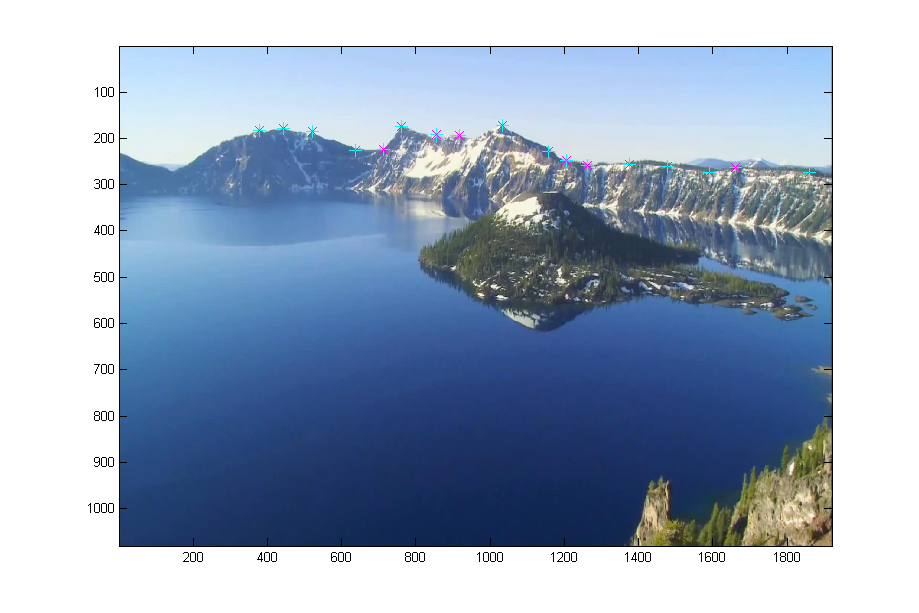
\includegraphics[height=3.5in]{sfmResults1/photoLeft_topRidgePoints.png}
\caption{Triangulation Points along the mountain peaks}
\end{figure}
\begin{figure}[H]
\centering
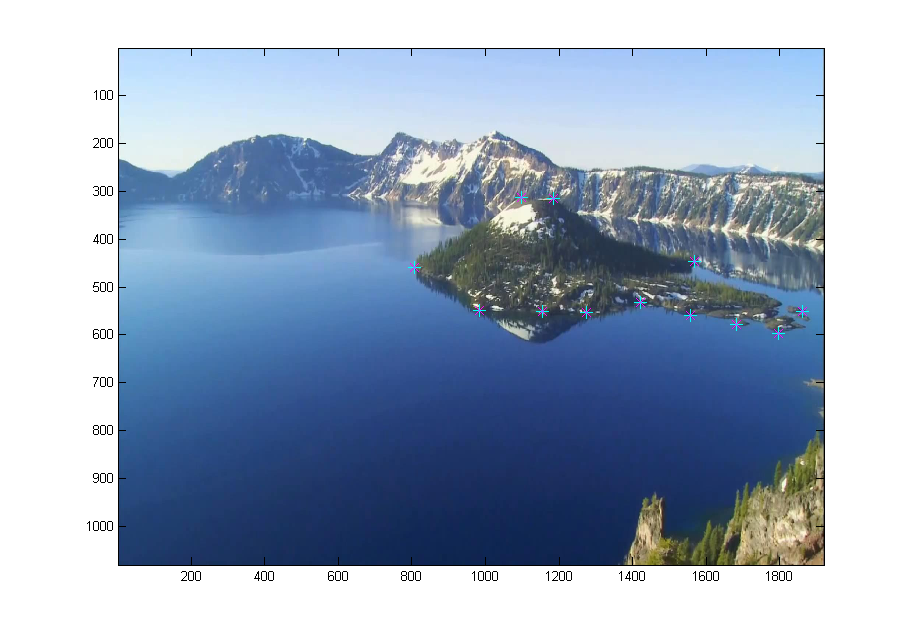
\includegraphics[height=3.5in]{sfmResults1/photoLeft_wizardIslandPoints.png}
\caption{Triangulation Points along Wizard Island}
\end{figure}

\newpage

Here is the right camera shot with the triangulation points.
\begin{figure}[H]
\centering
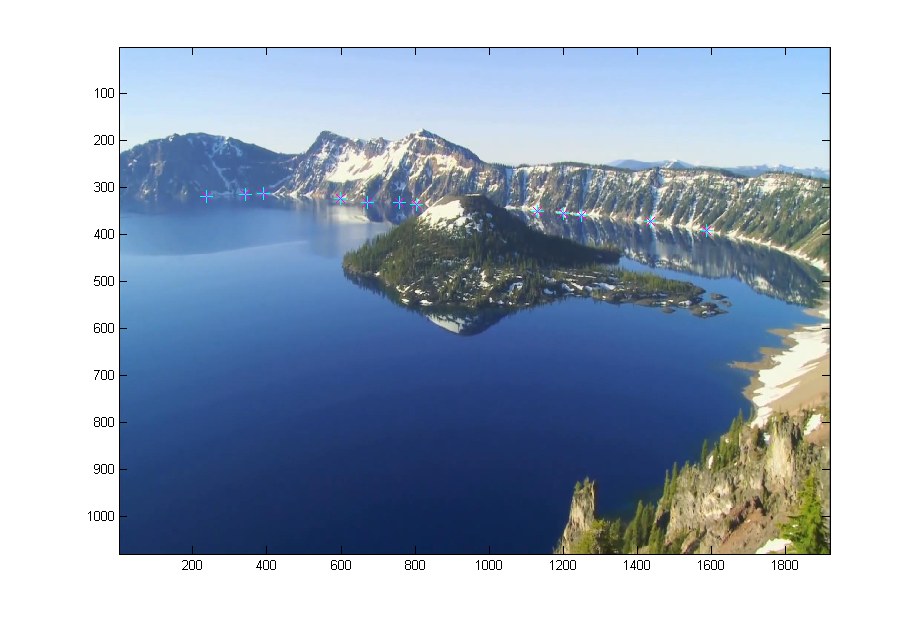
\includegraphics[height=3.5in]{sfmResults1/photoRight_lakeRidgePoints.png}
\caption{Triangulation Points along the lake}
\end{figure}
\begin{figure}[H]
\centering
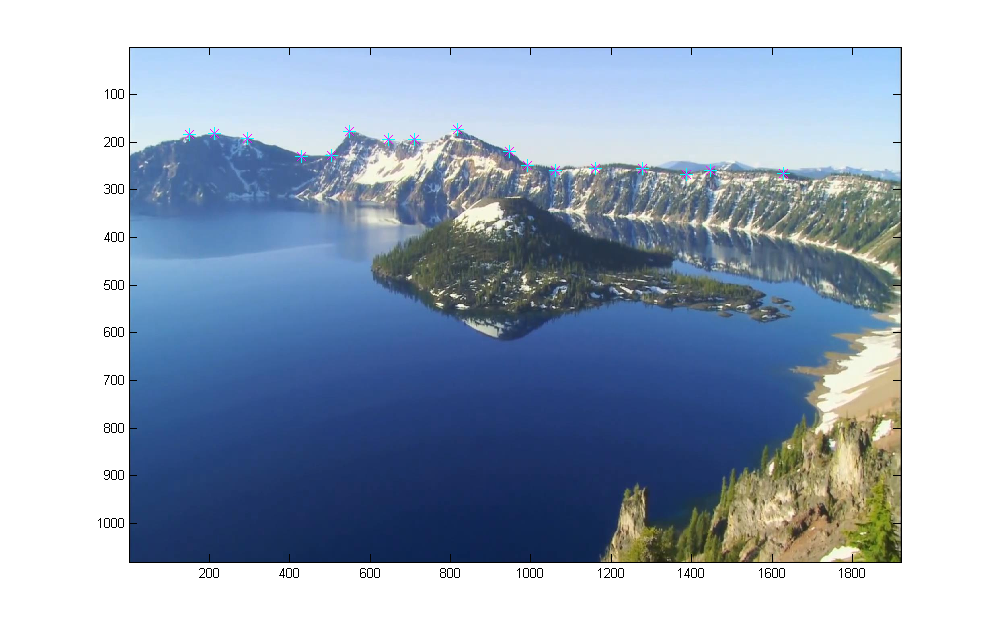
\includegraphics[height=3.5in]{sfmResults1/photoRight_topRidgePoints.png}
\caption{Triangulation Points along the mountain peaks}
\end{figure}
\begin{figure}[H]
\centering
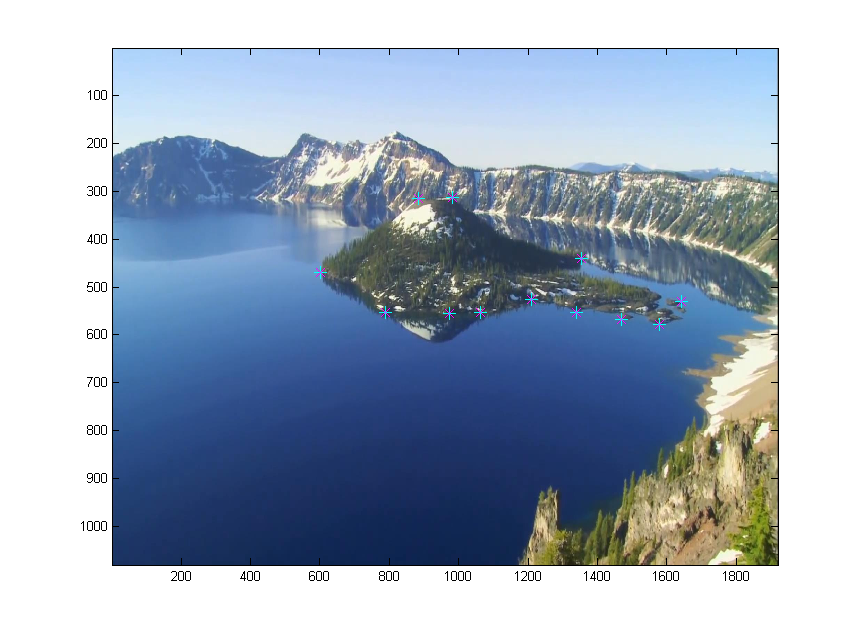
\includegraphics[height=3.5in]{sfmResults1/photoRight_wizardIslandPoints.png}
\caption{Triangulation Points along Wizard Island}
\end{figure}

\newpage

Here is a 3D visualization of the approximated 3D Points. The blue x marks represent the $z=0$ plane. The red circles represent the points on the peak of the mountains in the background. The green circles represent the points along the surface of the lake. The blue circles represent the points along Wizard Island. 
\begin{figure}[H]
\centering
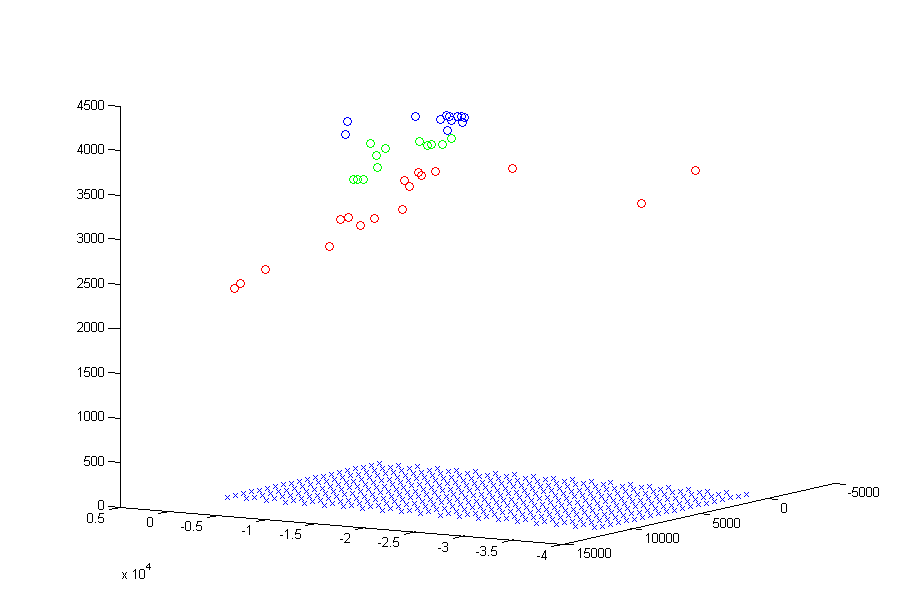
\includegraphics[height=3.5in]{sfmResults1/triangulationAttempt.png}
\caption{3D Reconstruction Points}
\end{figure}
\begin{figure}[H]
\centering
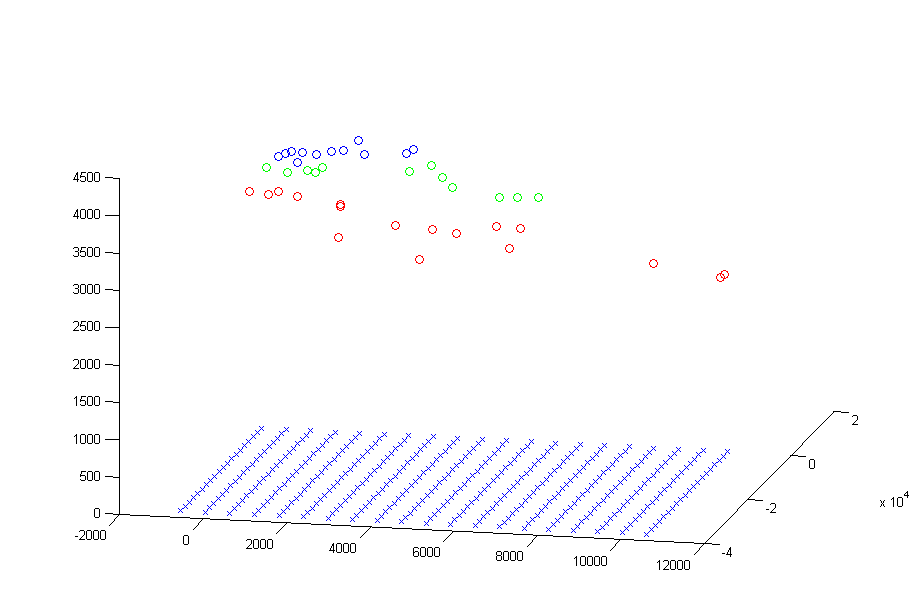
\includegraphics[height=3.5in]{sfmResults1/triangulationAttempt2.png}
\caption{3D Reconstruction Points}
\end{figure}
\begin{figure}[H]
\centering
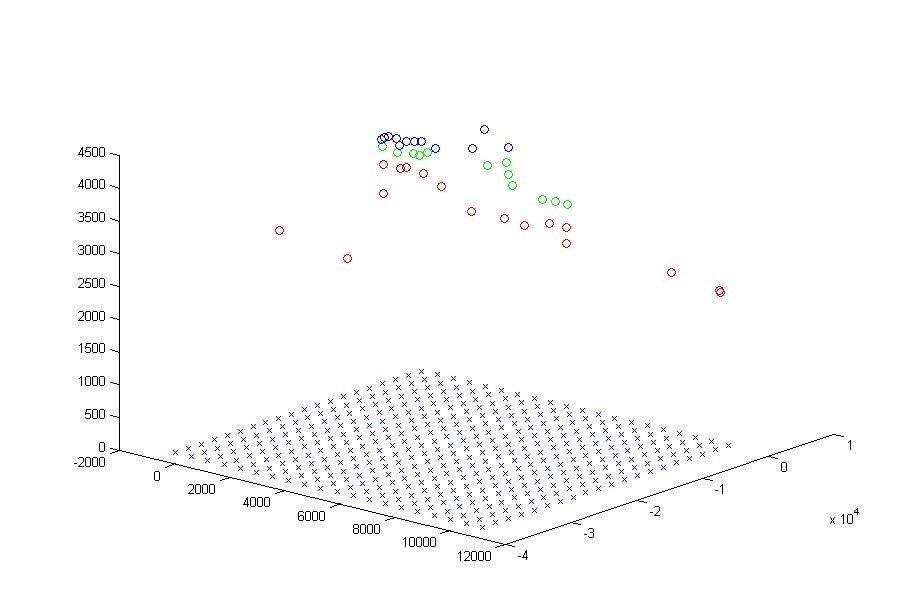
\includegraphics[height=3.5in]{sfmResults1/triangulationAttempt3.png}
\caption{3D Reconstruction Points}
\end{figure}
\begin{figure}[H]
\centering
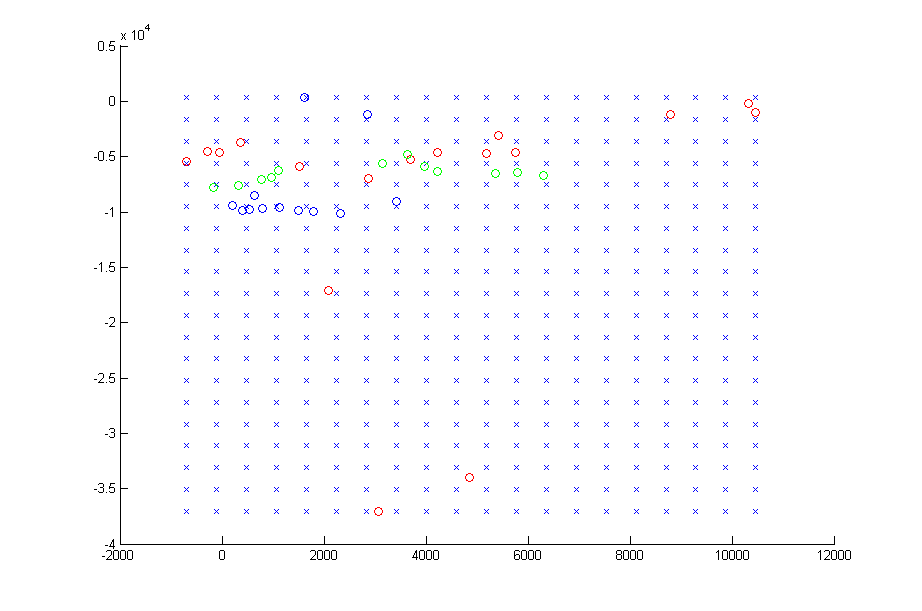
\includegraphics[height=3.5in]{sfmResults1/triangulationAttempt4.png}
\caption{3D Reconstruction Points}
\end{figure}

As can be observed, the reconstruction proved to be quite poor and while there is some shape, it is not at all what we expect. There are a few likely reasons for this. The biggest challenge is the immense size of what I am trying to image. Because the pictures were taken thousands of feet away from the object, it is likely that the image is relatively flat from the camera's perspective and thus when we move the camera, it does not pick up on much depth. The other major challenge was picking points accurately. Because the object was thousands of feet away, a single pixel error meant the estimate would be off by hundreds of feet. The aggregate of all these errors could easily have a major impact on the camera parameter estimates and final reconstruction. 

\newpage

\subsection{Triangulation using SIFT Matches}

In order to improve my triangulation points, I decided to run SIFT using VLFeat and use the best 100 matches. I used the following mask to make sure points were selected on wizard island or the background mountains. 
\begin{figure}[H]
\centering
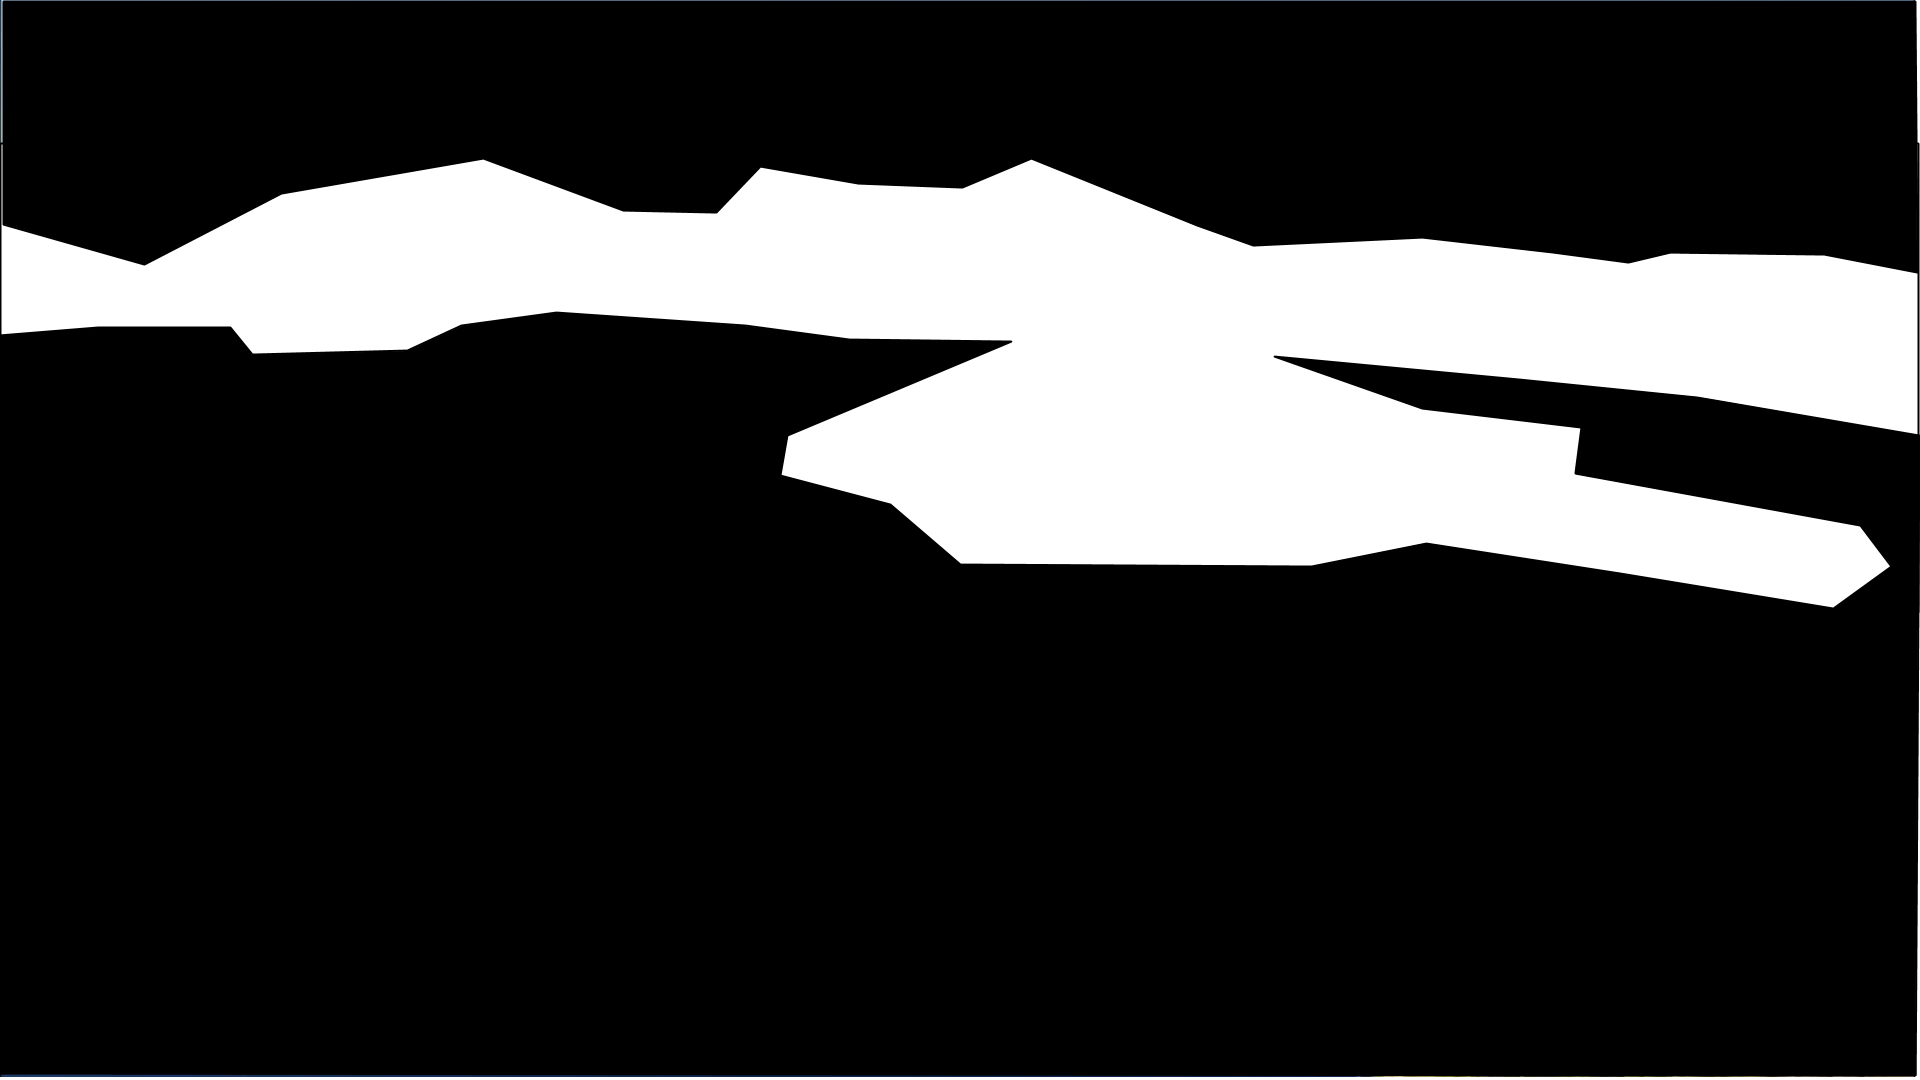
\includegraphics[width=\columnwidth]{sfmResults1/Shot4Mask.png}
\caption{Mask for selecting points}
\end{figure}

\newpage

These were the SIFT features and matches computed:
\begin{figure}[H]
\centering
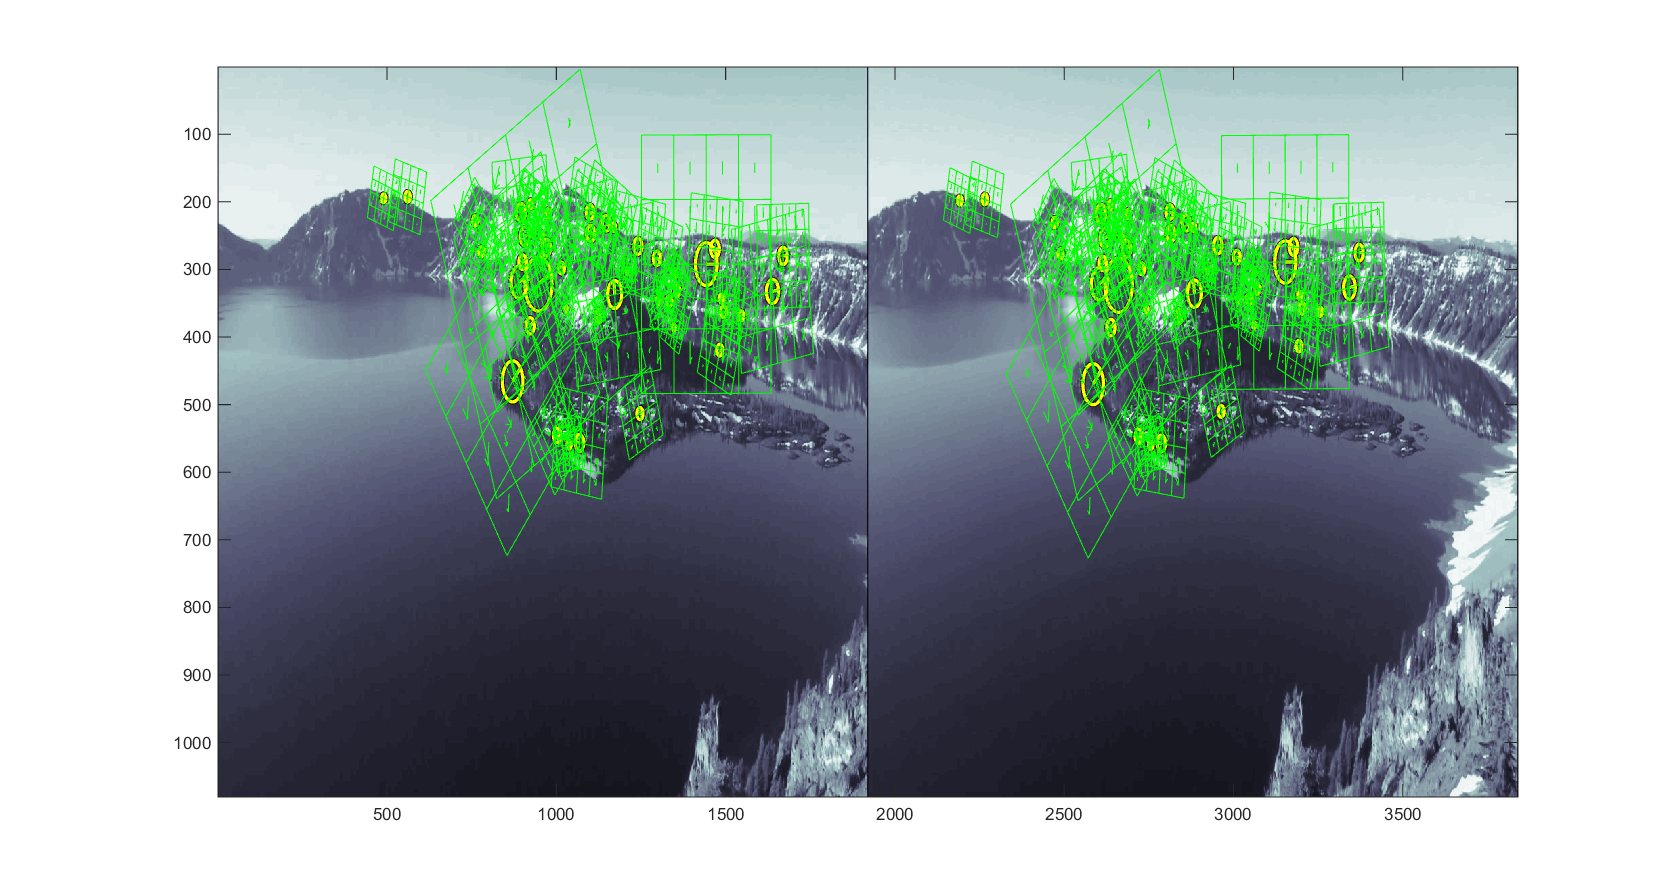
\includegraphics[width=\columnwidth]{sfmResults1/siftMatchesVLFeat1.png}
\caption{SIFT Features}
\end{figure}
\begin{figure}[H]
\centering
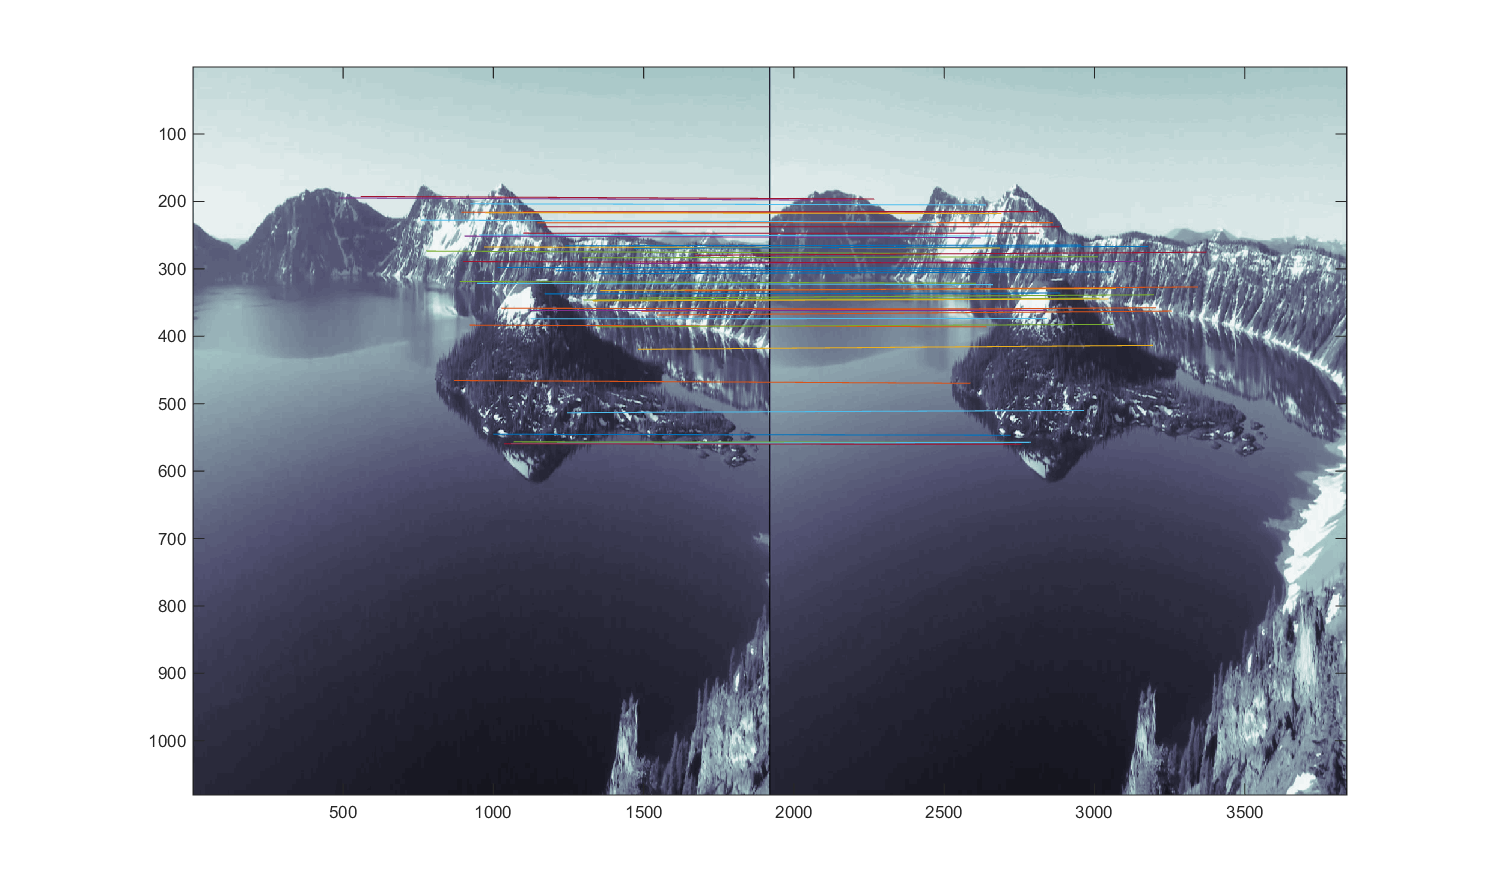
\includegraphics[width=\columnwidth]{sfmResults1/siftMatchesVLFeat2.png}
\caption{SIFT matches between images}
\end{figure}

\newpage

After running those points through the triangulation code, here was my reconstruction. As before, the blue x marks represent the $z=0$ plane. The red circles represent the SIFT points in 3D:
\begin{figure}[H]
\centering
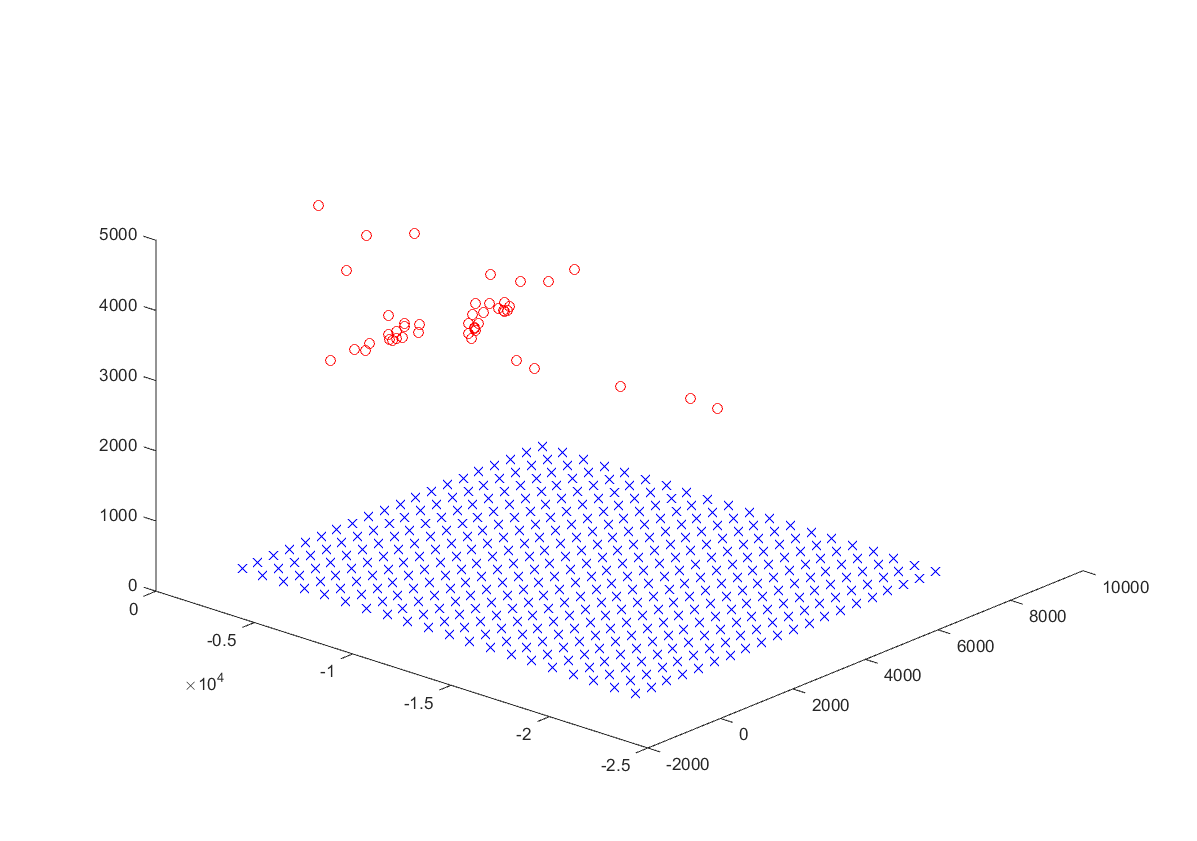
\includegraphics[height=3.5in]{sfmResults1/triangulationAttemptSIFT1.png}
\caption{3D Reconstruction Points}
\end{figure}
\begin{figure}[H]
\centering
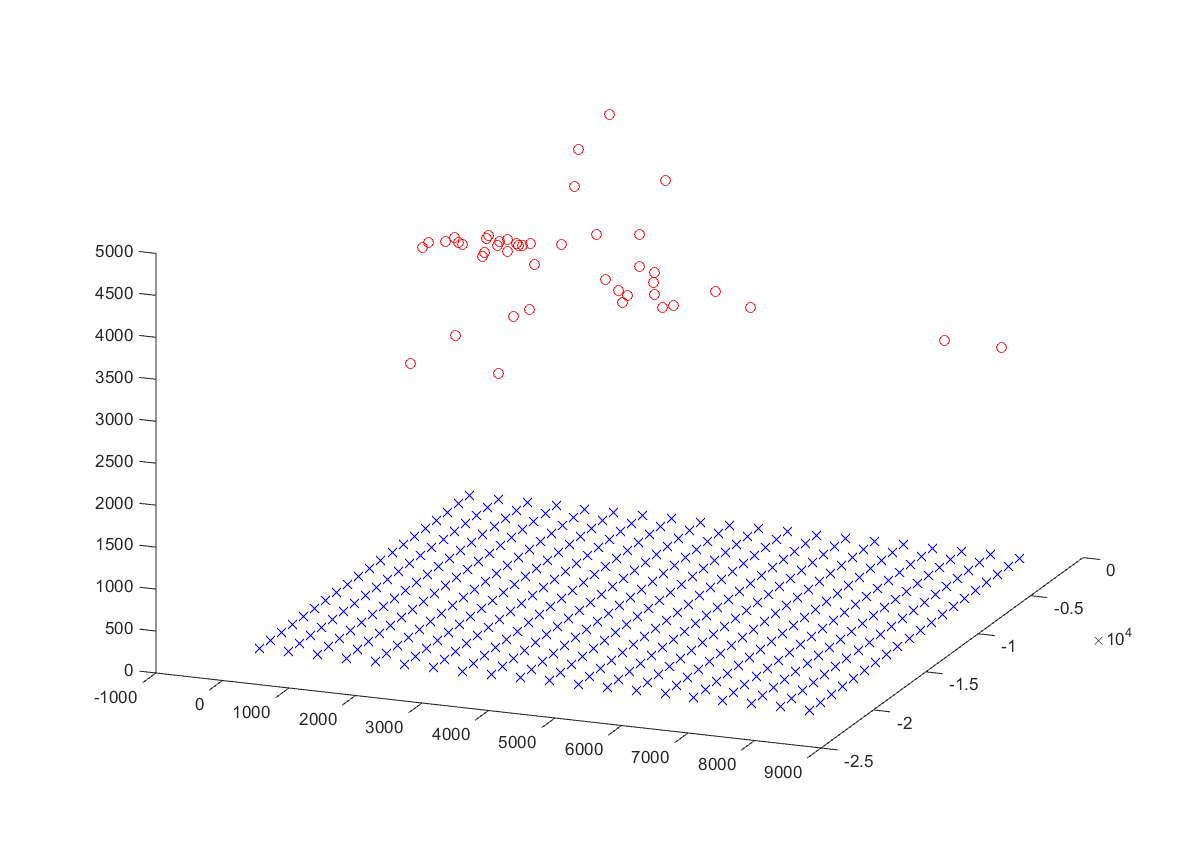
\includegraphics[height=3.5in]{sfmResults1/triangulationAttemptSIFT2.png}
\caption{3D Reconstruction Points}
\end{figure}
\begin{figure}[H]
\centering
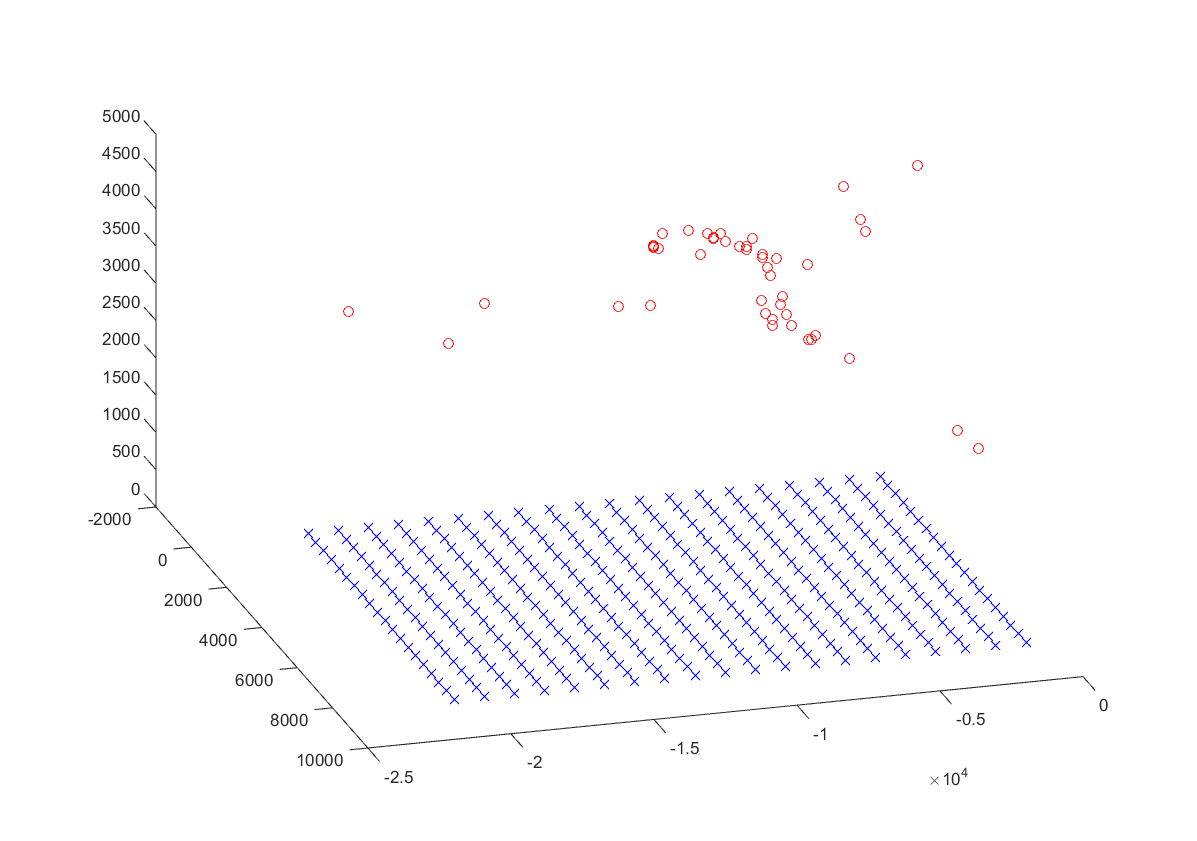
\includegraphics[height=3.5in]{sfmResults1/triangulationAttemptSIFT3.png}
\caption{3D Reconstruction Points}
\end{figure}
\begin{figure}[H]
\centering
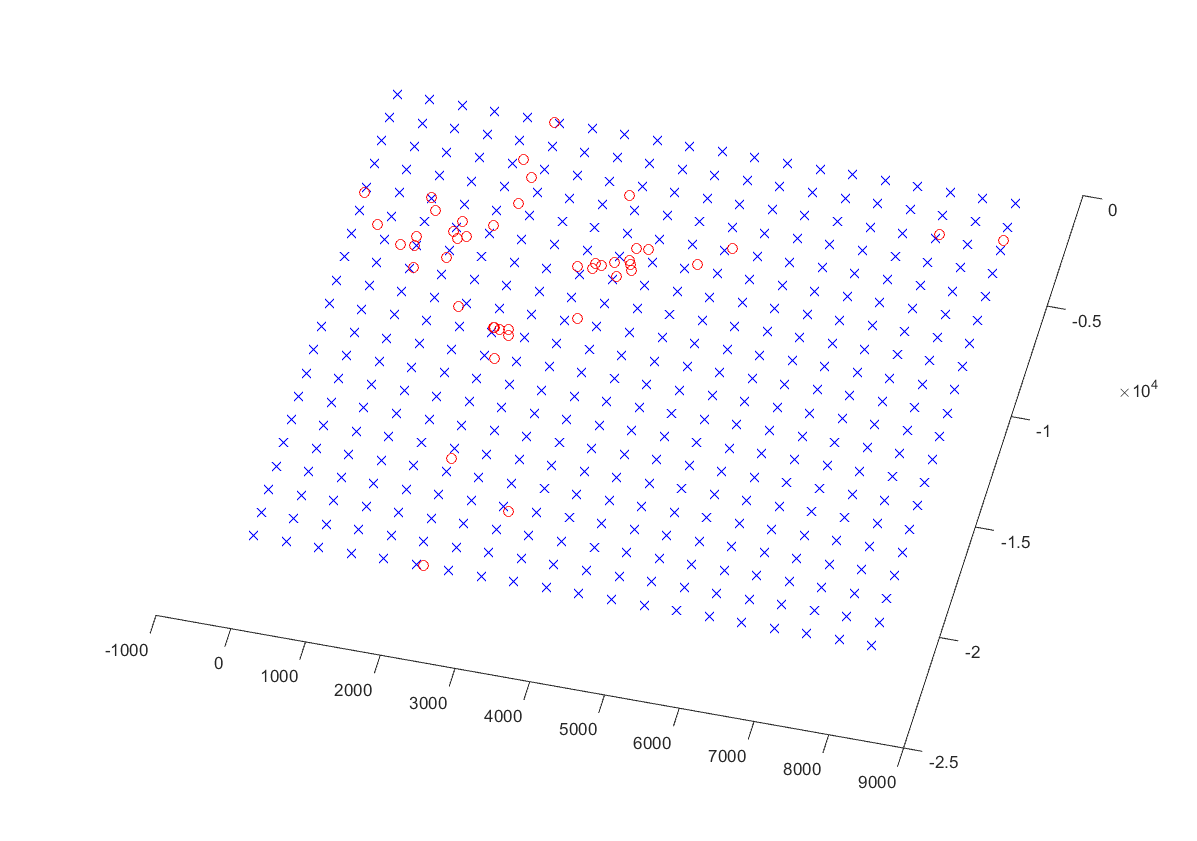
\includegraphics[height=3.5in]{sfmResults1/triangulationAttemptSIFT4.png}
\caption{3D Reconstruction Points}
\end{figure}

As before, the reconstruction proved to be relatively poor. This is likely due to the same reasons as before. Using SIFT does reduce the possible error that stems from being inaccurate by a few pixels when selecting points, provided that those points were good matches in the first place. Issues estimating depth still appear since our camera did not move much as compared to the size of the objects involved.   

\newpage

\subsection{VisualSFM Reconstruction Attempt}

With the shots that I used, there was little to no translational motion and thus SFM did not work well. I found this out the hard way when running Visual SFM. In any case, this is what VisualSFM was able to accomplish with these shots. It picked up on the following features:
\begin{figure}[H]
\centering
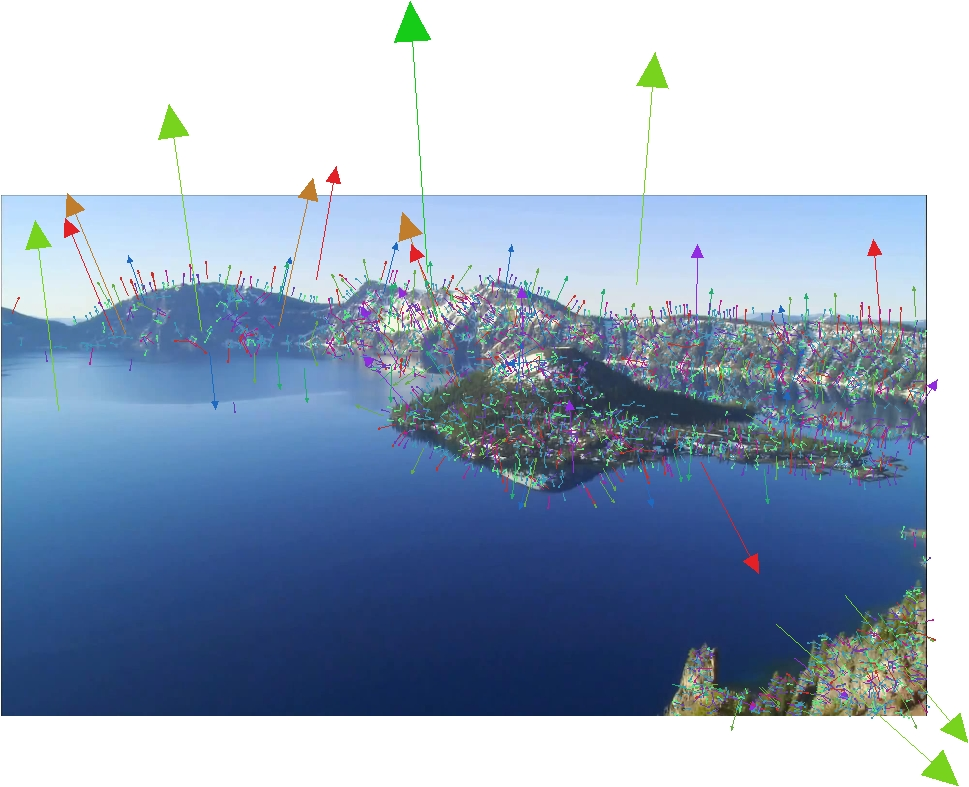
\includegraphics[height=3.5in]{sfmResults1/shotFeatures_4.jpg}
\caption{SIFT Features for left camera shot found using Visual SFM}
\end{figure}
\begin{figure}[H]
\centering
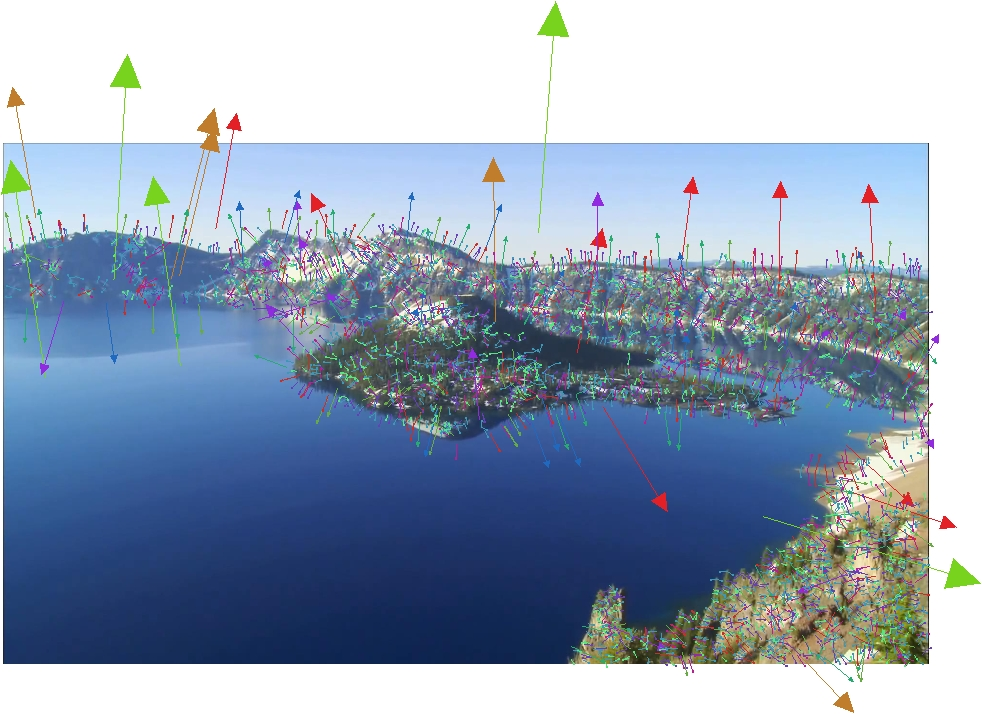
\includegraphics[height=3.5in]{sfmResults1/shotFeatures_26.jpg}
\caption{SIFT Features for right camera shot found using Visual SFM}
\end{figure}
\newpage
It also found the following matches between two of the shots. Matches between other pairs were similar. 
\begin{figure}[H]
\centering
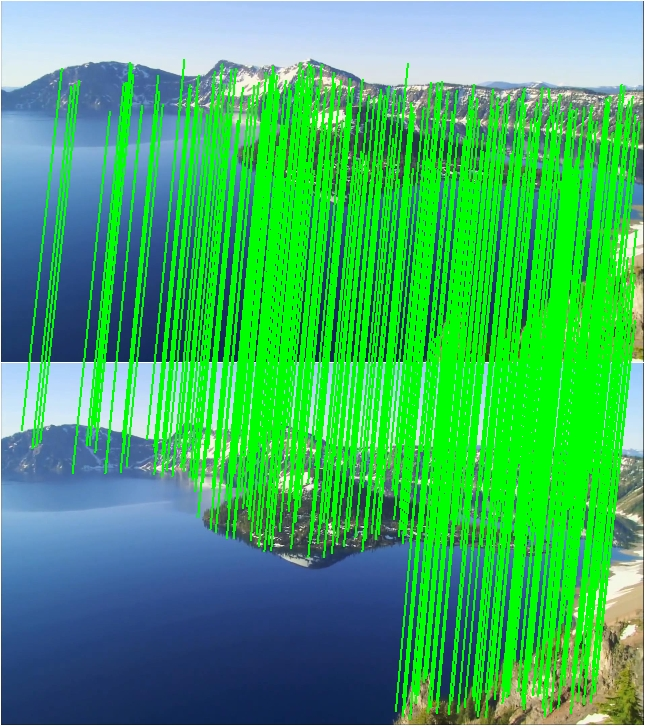
\includegraphics[width=\columnwidth]{sfmResults1/shot14_26_siftMatches.jpg}
\caption{SIFT Matches found between images using VisualSFM}
\end{figure}

\newpage

However, the points obtained in the 3D reconstruction had little to no pattern at all. All the cameras were also in one spot. In addition to the obstacles already mentioned, there was an additional issue in that VisualSFM detected points on the lake and points in the sky. Those points do not have good structure to them, thus they likely skewed the final results. 

\newpage

\section{Reconstruction of Wizard Island Scene}

I found another scene where they show Wizard Island up close and then it cuts to a shot of Wizard Island where the camera is behind the original shot and from a different persective. I decided to put these frames through Visual SFM to see if the translational motion would produce better SFM results. Here is the 3D Reconstruction computed using VisualSFM of those frames. 

\begin{figure}[H]
\centering
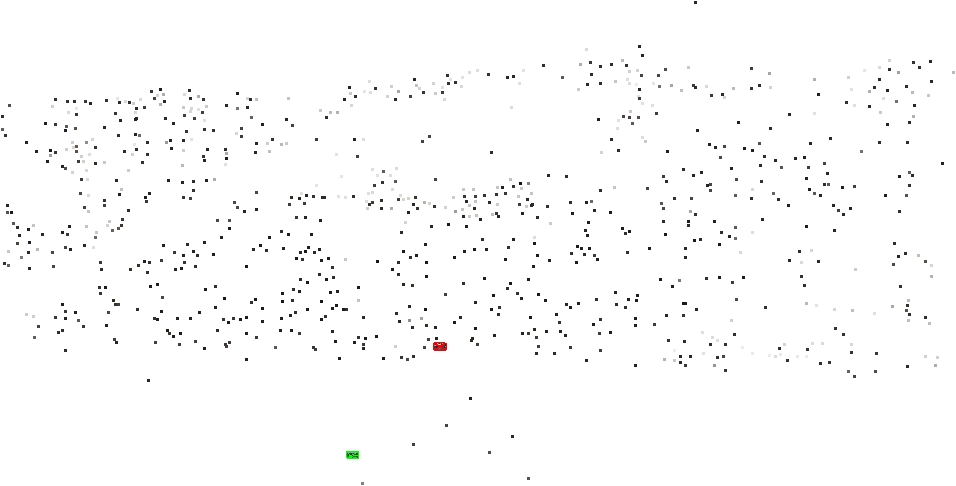
\includegraphics[height=3.5in]{sfmResults3/3Dreconstruction1.jpg}
\caption{3D Reconstruction Points}
\end{figure}
\begin{figure}[H]
\centering
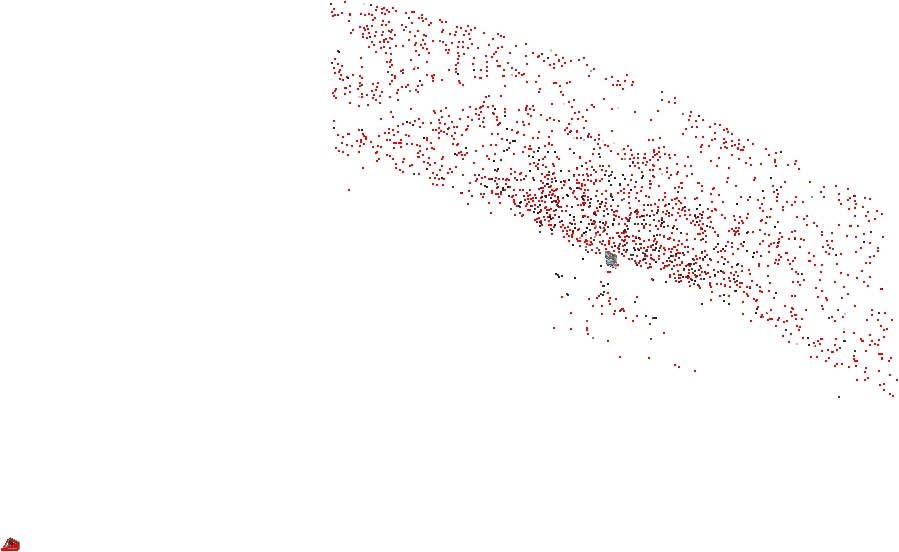
\includegraphics[height=3.5in]{sfmResults3/3DreconstructionFromMany1.jpg}
\caption{3D Reconstruction Points}
\end{figure}
\begin{figure}[H]
\centering
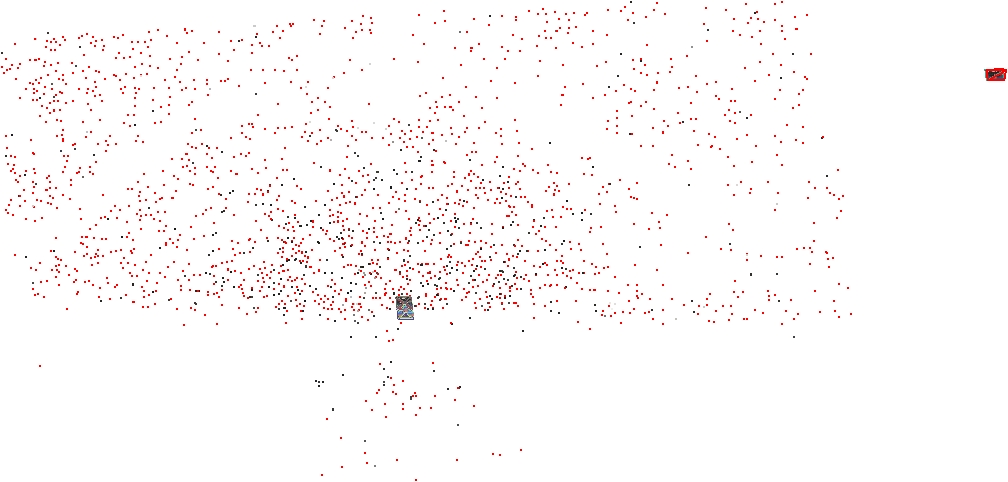
\includegraphics[height=3.5in]{sfmResults3/3DreconstructionFromMany2.jpg}
\caption{3D Reconstruction Points}
\end{figure}

\newpage 

As can be observed, VisualSFM did indeed detect that one of the pictures was taken from a vantage point which was behind the other picture. It also seemed to reconstruct the 2D shape of Wizard Island relatively well. Unfortunately, there was almost no depth to each of the points. 

\newpage

\section{Conclusion}

After attempting to reconstruct mountain scenes using photos, I have a new appreciation for topographic maps and elevation data sets. Capturing the depth when looking at a mountain seems to be one of the biggest challenges as none of my reconstruction methods were remotely accurate with it. The lack of distance between vantage points was a likely culprit in why the depth calculations were very inaccurate. Additionally, in a picture of a mountain, there are patches of trees, rocks, and snow and the patches can look quite similar. Thus the probability of selecting bad point matches is relatively high. \\
\\
In the end, I was not close to being able to construct something similar to what Google Earth provides. If I do want to make a 3D reconstruction of a mountain, then I will use the entire elevation data set of it from the United States Geological Survey (USGS). This way it will likely be much more detailed and accurate than a stereo reconstruction. This is likely the method employed by Google Earth. 

\section{Attached Code}

\subsection{Matlab Code and Data}

The code getPoints.m was the script used to attempt the 3D reconstruction of the shot from Merriam Point. The code siftMatching.m computed the SIFT matches using VLFeat. \\
\\
The folder entitled data contains the input I used. The subfolder merriamPointData contains the input images that were used in the 3D reconstruction of Merriam Point. The subfolder wizardIslandPicsForVisualSFM contains the images that were put through VisualSFM for the reconstruction of the second shot. 

\newpage

\section{References}

\subsection{Video Sources}

The shots of Merriam Point were frames in the following video at time 5:11
\begin{verbatim}
https://www.youtube.com/watch?v=qbH5--nwxdk
\end{verbatim}
The shots of Wizard Island were frames in the following video at time 3:48
\begin{verbatim}
https://www.youtube.com/watch?v=VImqiFWRWZ4
\end{verbatim}

\subsection{Geographic Data}

The topographic maps I used were sections of the maps Crater Lake West and Crater Lake East from the United States Geological Survey. The map showing the exact elevations is a section of the standard map of Crater Lake National Park from the National Park Service. 



\end{document}








